%% Template para dissertacao/tese na classe UFBAthesis
%% versao 1.0
%% (c) 2005 Paulo G. S. Fonseca
%% (c) 2012 Antonio Terceiro
%% (c) 2014 Christina von Flach
%% www.dcc.ufba.br/~flach/ufbathesis

%% Carrega a classe ufbathesis
%% Opcoes: * Idiomas
%%           pt   - portugues (padrao)
%%           en   - ingles
%%         * Tipo do Texto
%%           bsc  - para monografias de graduacao
%%           msc  - para dissertacoes de mestrado (padrao)
%%           qual - exame de qualificacao de mestrado
%%           prop - exame de qualificacao de doutorado
%%           phd  - para teses de doutorado
%%         * Media
%%           scr  - para versao eletronica (PDF) / consulte o guia do usuario
%%         * Estilo
%%           classic - estilo original a la TAOCP (deprecated) - apesar de deprecated, manter esse.
%%           std     - novo estilo a la CUP (padrao)
%%         * Paginacao
%%           oneside - para impressao em face unica
%%           twoside - para impressao em frente e verso (padrao)

% Atenção: Manter 'classic' na declaracao abaixo:
\documentclass[qual, classic, a4paper]{ufbathesis}

%% Preambulo:
\usepackage[utf8]{inputenc}

%\usepackage[authoryear]{natbib}
\usepackage{graphicx}
\usepackage{lipsum}
\usepackage{hyphenat}
\usepackage[usenames, dvipsnames, table]{xcolor}
\usepackage{booktabs}
\usepackage{pifont}
\usepackage{multirow}
\usepackage{listings} 
\usepackage{colortbl}
\usepackage{xfrac}
\usepackage[FIGTOPCAP]{subfigure}
\usepackage{tabularx}
\usepackage{ragged2e}
\usepackage{acronym}
\usepackage{float}
\usepackage{todonotes}
\usepackage{amssymb}
\usepackage{placeins}
\usepackage{arydshln}

\presetkeys%
    {todonotes}%
    {inline,backgroundcolor=yellow}{}
    
\usepackage{blindtext}

\usepackage{tikz}
\usetikzlibrary{arrows,shapes,positioning,shadows,trees}

% Siglas
\acrodef{AM}[AM]{{Aprendizado de Máquina}}
\acrodef{DE}[DE] {{Distância Euclidiana}}
\acrodef{FCD}[FCD] {{\textit {Fluxo de Dados Contínuos}}}
\acrodef{DN}[DN] {{\textit {Detecção de Novidade}}}

% Universidade
\university{Universidade Federal da Bahia}

% Endereco (cidade)
\address{Salvador}

% Instituto ou Centro Academico
\institute{Instituto de Matem\'{a}tica}

% Nome da biblioteca - usado na ficha catalografica
\library{Biblioteca Reitor Mac\^{e}do Costa}

% Programa de pos-graduacao
\program{Programa de P\'{o}s-Gradua\c{c}\~{a}o em Ci\^{e}ncia da Computa\c{c}\~{a}o}

% Area de titulacao
\majorfield{Ci\^{e}ncia da Computa\c{c}\~{a}o}

% Titulo da dissertacao
\title{Aplicando redes de função de base radial para detecção de mudanças de conceito em fluxos contínuos de dados}

% Data da defesa
% e.g. \date{19 de fevereiro de 2013}
\date{03 de Abril de 2019}
% e.g. \defenseyear{2013}
\defenseyear{2019}

% Autor
% e.g. \author{Jose da Silva}
\author{Ruivaldo Azevedo Lobão Neto}

% Orientador(a)
% Opcao: [f] - para orientador do sexo feminino
% e.g. \adviser[f]{Profa. Dra. Maria Santos}
\adviser{Ricardo Ara\'{u}jo Rios}

% Orientador(a)
% Opcao: [f] - para orientador do sexo feminino
% e.g. \coadviser{Prof. Dr. Pedro Pedreira}
% Comente se nao ha co-orientador
%\coadviser{Nome Completo do CO-ORIENTADOR}

%% Inicio do documento
\begin{document}

\pgcompfrontpage

%% Parte pre-textual
\frontmatter

\pgcomppresentationpage

%%%%%%%%%%%%%%%%%%%%%%%%%
% Ficha catalografica
%%%%%%%%%%%%%%%%%%%%%%%%%

%\authorcitationname{Silva, Mirlei Moura da } % e.g. Terceiro, Antonio Soares de Azevedo
%\advisercitationname{Sobrenome, Nome do ORIENTADOR} % e.g. Chavez, Christina von Flach Garcia
%\coadvisercitationname{Sobrenome, Nome do CO-ORIENTADOR} % e.g. Mendonca, Manoel Gomes de
%\catalogtype{Disserta\c{c}\~{a}o (Mestrado)} % e.g. ou ``Tese (Doutorado)''

%\catalogtopics{1. Primeira palavra-chave. 2. Segunda palavra-chave. 3. Terceira palavra-chave} % Listar palavras-chave do trabalho para a FICHA CATALOGRAFICA}, por exemplo, ``1. Complexidade Estrutural. 2. Qualidade de Software 3. Engenharia de Software''
%\catalogcdd{XXX.XX} % e.g.  XXX.XX (número nesse formato serah dado pela biblioteca)
%\catalogcdu{XXX.XX.XXX} % e.g.  XXX.XX.XXX (idem) 
%\catalogingsheet

%%%%%%%%%%%%%%%%%%%%%
% Termo de aprovacaoo
%%%%%%%%%%%%%%%%%%%%%

\approvalsheet{Salvador, 03 de Abril de 2019}{
   \comittemember{Prof. Dr. Ricardo Araújo Rios}{UFBA}  
   %\comittemember{Profa. Dr...}{UFBA}
   %\comittemember{Prof. Dr...}{USP} 
}
   % Para mestrado, apenas 3.
   % \comittemember{Prof. Dr. Professor 4}{Universidade HJKL}
   % \comittemember{Profa. Dra. Professora 5}{Universidade QWERTY}

%%%%%%%%%%%%%%%%%%%%%%%%%%%%%%%%%%%%%%%% 
% Dedicatoria, Agradecimentos, Epigrafe
%%%%%%%%%%%%%%%%%%%%%%%%%%%%%%%%%%%%%%%%

% Comente para ocultar
%\begin{dedicatory}
%DIGITE A DEDICATORIA AQUI
%\end{dedicatory}

% Agradecimentos
% Se preferir, crie um arquivo `a parte e o inclua via \include{}
%\acknowledgements
%DIGITE OS AGRADECIMENTOS AQUI

% Epigrafe
%\begin{epigraph}[NOTA]{AUTOR}
%DIGITE AQUI A CITACAO
%\end{epigraph}

%%%%%%%%%%%%%%%%%%%%%
% Resumo 
%%%%%%%%%%%%%%%%%%%%%
\resumo

\blindtext

% Palavras-chave do resumo em Portugues
\begin{keywords}
    Aprendizado de Máquina, Fluxos Contínuos de Dados, Mudanças de Conceito, Redes de Função de Base Radial, Não supervisionado
\end{keywords}

\abstract

\blindtext

% Palavras-chave do resumo em Ingles
\begin{keywords}
    Machine Learning, Data Streams, Concept Drift, Radial Basis Function Networks, RBF Network, Unlabeled
\end{keywords}

%%%%%%%%%%%%%%%%%%%
% Sumario / Indice
%%%%%%%%%%%%%%%%%%%

% Comente para ocultar
\tableofcontents

% Lista de figuras
% Comente para ocultar
\listoffigures

% Lista de tabelas
% Comente para ocultar
\listoftables

%% Parte textual
\mainmatter

% Eh aconselhavel criar cada capitulo em um arquivo separado, digamos
% "capitulo1.tex", "capitulo2.tex", ... "capituloN.tex" e depois
% inclui-los com:
% \include{capitulo1}
% \include{capitulo2}
% ...
% \include{capituloN}
%
% Importante: 
% Use \xchapter{}{} ao inves de \chapter{}; se não quiser colocar texto antes do inicio do capitulo, use \xchapter{texto}{}.

%%%
\xchapter{Introdução}{} \label{introducao}

\section{Contexto e Motivação}

Nos últimos anos, o volume de dados produzidos por sistemas computacionais tem crescido de forma acentuada.
%
Esse crescimento foi favorecido por avanços tecnológicos recentes, como  
a pervasividade dos dispositivos móveis,
a popularização das redes sociais e 
a expansão da internet das coisas \cite{Cohen:BigData:2009:MSN:1687553.1687576}.
%
A dimensão desse aumento é verificada em \cite{idc_report}, 
no qual se estima que, entre os anos de 2014 e 2020,
a quantidade de informações produzidas anualmente irá aumentar de 4,4 zettabytes (trilhões de gigabytes) para 44 zettabytes.

Parte significativa dessas informações é produzida na forma de sequências ininterruptas e potencialmente infinitas \cite{Aggarwal:2006:DSM:1196418}.
%
Na literatura, sequências com essas características são denominadas Fluxos Contínuos de Dados (FCDs) e estão presentes em diversos domínios de aplicação, por exemplo:
monitoramento do mercado financeiro \cite{ZHOU:2015},
acompanhamento de tráfico rodoviário \cite{Wang:2015:EOV:2843092.2843464}, 
gerenciamento de redes de telecomunicação \cite{delattre2015method}, 
análise de sentimento em tempo real \cite{KRANJC2015187} e 
sistemas de prevenção e identificação de intrusos \cite{KENKRE:PAI:COLACO:2015}.

Para extrair informações úteis dessa grande quantidade de dados, 
pesquisadores têm aplicado técnicas da área de Aprendizado de Máquina (AM), 
a qual estuda algoritmos que melhoram seu desempenho conforme ganham experiência \cite{Mitchell:1997:ML:541177}.
%
Entretanto, as estratégias tradicionais de aprendizado de máquina têm aplicação limitada para contextos com fluxos contínuos de dados, 
pois nesses cenários os algoritmos devem atender a severas restrições de tempo de execução e de uso dos recursos computacionais \cite{bifet2009data}.

Além dessas limitações, 
as técnicas de aprendizado de máquina, 
quando aplicadas em contextos com fluxos contínuos, 
também devem lidar com variações na distribuição dos dados ou no contexto do processo gerador.
%
Essas alterações são denominadas Mudanças de Conceito \cite{Gama:2010:KDD:1855075} e 
a sua ocorrência pode impactar a acurácia do algoritmo.

Inicialmente, a atualização periódica do modelo foi utilizada como estratégia para evitar a perda de acurácia causada por tais mudanças.
%
Contudo, esta solução é pouco sofisticada e computacionalmente custosa.
% 
Diante disso, pesquisadores propuseram técnicas de detecção de mudanças de conceito baseadas em monitoramento \cite{Gama:2014:SCD:2597757.2523813}.
% 
Estes métodos identificam o momento exato da mudança, permitindo que o modelo de decisão seja atualizado somente quando necessário.
%
Exemplos de algoritmos baseados nesta abordagem, incluem: 
DDM \cite{GamaMCR04}, EDDM \cite{EDDM},  
ADWIN \cite{BifetG07}, ECDD \cite{Ross:2012:EWM:2076039.2076307}, 
PL \cite{Bach:PL:2008}, FCWM \cite{FCWM} e STEPD \cite{STEPD}.

Entretanto, as técnicas baseadas em monitoramento necessitam que o rótulo correto de cada exemplo esteja disponível.
%
Em muitos cenários, o tempo ou o custo para obter esses rótulos é proibitivo \cite{Aggarwal:2006:DSM:1196418}.
%
Consequentemente, foram desenvolvidos novos algoritmos independentes de rótulos.
Nestes métodos, a detecção se baseia na identificação de exemplos que não se enquadram na estrutura dos dados \cite{Spinosa:2007:OCA:1244002.1244107}.
% 
Essa análise é implementada com base em técnicas de agrupamento, detecção de \textit{outliers} e medidas de dissimilaridade \cite{Ryu:Kantardzic:2012}.
%
Os seguintes algoritmos são exemplos desta metodologia:
OLINDDA \cite{Spinosa:2007:OCA:1244002.1244107},
MINAS \cite{Faria:2013:NDA:2480362.2480515},
ECSMiner \cite{Masud:2011:CNC:1978259.1978529} e 
GC3 \cite{Sethi2016b:GC3}.

Todavia, segundo \citeonline{Aggarwal:2006:DSM:1196418},
as técnicas de detecção de mudanças de conceito propostas apresentam limitações ao serem aplicadas em cenários com fluxos contínuos de dados.
% 
Os algoritmos dependentes de rótulo se tornam inviáveis, por causa do custo e do tempo necessário para obter os rótulos corretos.
%
Enquanto as técnicas independentes têm dificuldade em atender as severas restrições de tempo de execução e de uso dos recursos computacionais desses cenários.

Visando resolver essas limitações, 
este projeto de mestrado discute uma abordagem baseada em redes de função de base radial 
para detecção de mudanças de conceito em fluxos contínuos de dados.
A metodologia proposta se diferencia por detectar as mudanças em tempo de execução, de forma computacionalmente eficiente e independente de rótulos.

\section{Hipótese e Objetivo}

Com base nas observações citadas anteriormente, a seguinte hipótese foi formulada:

\begin{center}
\textit{``
A aplicação de redes de função de base radial a fluxos contínuos de dados permite a detecção de mudanças de conceito em tempo de execução, de forma computacionalmente eficiente e independente de rótulos.
''}
\end{center}

Assim, o objetivo deste trabalho de mestrado será a validação desta hipótese.
%
Para atingir este objetivo, será desenvolvido um método para detecção de mudanças de conceito baseado em redes de função de base radial.
%
A técnica proposta será validada através de comparações com o estado da arte.
%
Os dados utilizados durante a validação serão divididos em dois conjuntos.
%
Um conjunto formado por dados sintéticos, que permitirão uma análise detalhada da abordagem, uma vez que as características e os comportamentos dos fluxos serão conhecidos.
%
O outro conjunto será composto por dados obtidos a partir de sistemas computacionais utilizados na indústria, visando apresentar uma aplicação prática para a solução proposta. 

O restante deste projeto está organizado conforme a seguinte estrutura: 
%
O \textbf{Capítulo \ref{revisao_bibliografica}} apresenta uma revisão bibliográfica dos principais conceitos utilizados neste trabalho como, por exemplo, fluxos contínuos de dados e aprendizado de máquina, mudança de conceito e redes de função de base radial; 
%
No \textbf{Capítulo \ref{plano_pesquisa}} o plano de pesquisa é detalhado, identificando a metodologia que será aplicada na pesquisa e o cronograma de atividades. 
%
Por fim, o \textbf{Capítulo \ref{experimentos_iniciais}} apresenta um conjunto de experimentos preliminares e a análise dos resultados obtidos.

\xchapter{Revisão Bibliográfica}{} \label{revisao_bibliografica}
\section{Considerações Iniciais}

Este capítulo apresenta uma discussão geral sobre os principais conceitos utilizados neste projeto.
%
Inicialmente, será abordada a relação entre fluxos contínuos de dados e técnicas de aprendizado de máquina.
%
Em seguida, o fenômeno mudança de conceito e seus métodos de detecção são discutidos.
%
Posteriormente, as redes de função de base radial são detalhadas.
%
Por fim, são apresentados os trabalhos relacionados encontrados na literatura.

\section{Fluxos Contínuos de Dados e Aprendizado de Máquina}

Fluxos Contínuos de Dados (FCDs) podem ser definidos como sequências ininterruptas e potencialmente infinitas de eventos \cite{Aggarwal:2006:DSM:1196418}.
%
Nestes fluxos, os eventos ocorrem em alta frequência, sendo necessário processá-los em tempo real.
%
Além disso, por serem de tamanho potencialmente ilimitado, não é possível armazená-los de forma permanente em memória.
%

As características dos fluxos contínuos de dados implicam nas seguintes restrições aos algoritmos que os processam \cite{bifet2009data}:
%
\begin{enumerate}
    \item É impossível armazenar todos os dados do fluxo. Somente uma pequena parcela pode ser processada e armazenada, enquanto o restante é descartado;
    \item A velocidade de chegada dos eventos no fluxo exige que os elementos sejam processados em tempo real;
    \item A distribuição dos dados pode mudar com o tempo. Assim, os dados do passado podem se tornar irrelevantes ou mesmo prejudiciais para a descrição dos conceitos atuais.
\end{enumerate}

A área de Aprendizado de Máquina (AM) estuda algoritmos que melhoram o seu desempenho conforme ganham experiência \cite{Mitchell:1997:ML:541177}.
%
Esses algoritmos se dividem em duas categorias principais: 
%
não supervisionados (agrupamento ou \textit{clustering}) e supervisionados (classificação ou regressão).
%
Algoritmos de ambas as categorias foram adaptados para que pudessem ser aplicados em cenários com fluxos contínuos de dados.
%
As principais características de cada categoria e as especializações propostas serão discutidas a seguir.

As técnicas não supervisionadas realizam o agrupamento automático de dados segundo o seu grau de semelhança.
Essas técnicas têm como objetivo a formação de grupos com alta similaridade intragrupo e baixa similaridade intergrupo \cite{Jain:1988:ACD:46712}.
Os seguintes algoritmos são exemplos de técnicas não supervisionadas para cenários em lote:
K-Means \cite{Lloyd:2006:LSQ:2263356.2269955},
DBSCAN \cite{Ester:1996:DAD:3001460.3001507},
PAM \cite{kaufman:clustering1990} e 
OPTICS \cite{Ankerst:1999:OOP:304181.304187}.

De acordo com \citeonline{Gama:2010:KDD:1855075}, a principal dificuldade ao aplicar técnicas não supervisionadas em cenários com fluxos contínuos é a manutenção da qualidade e consistência dos grupos formados conforme novos dados são observados.
Portanto, é necessário que os algoritmos atuem de forma incremental, evoluindo os grupos formados ao longo do tempo \cite{Barbara:2002:RCD:507515.507519}.
Sendo assim, foram desenvolvidos métodos não supervisionados especializados para fluxos contínuos de dados.
Os seguintes trabalhos são exemplos dessas especializações:
CluStream \cite{Aggarwal:2003:FCE:1315451.1315460},
StreamKM++ \cite{Ackermann:2012:SCA:2133803.2184450},
DenStream \cite{Cao:Feng:Ester},
D-Stream \cite{Chen:Tu} e ClusTree \cite{Kranen:2011:CIM:2134350.2134352}.

Os algoritmos supervisionados realizam predições para novos exemplos utilizando um modelo criado a partir de uma base de treinamento \cite{Kotsiantis:2007:SML:1566770.1566773}.
Se a predição é categórica, entende-se como um problema de classificação.
Se a predição resulta em um valor numérico, trata-se de uma tarefa de regressão.
Exemplos de algoritmos supervisionados para cenários em lote, incluem:
árvores de decisão \cite{Breiman:Classification_Regression_Trees},
métodos baseados em regras, 
redes neurais e máquinas de vetores suporte (SVM) \cite{Vapnik1998}.

Segundo \citeonline{Gama:2010:LDS:1951990}, 
as técnicas supervisionadas tradicionais não podem ser aplicadas a contextos com fluxos contínuos de dados, 
pois estes métodos não contemplam as severas restrições de uso de memória e de tempo de execução desses cenários.
%
Dessa forma, 
novos algoritmos supervisionados foram propostos para esses contextos \cite{Domingos:2000:MHD:347090.347107, Bifet:2013:EDS:2480362.2480516, Wang:2003:MCD:956750.956778, Aggarwal:2004:DCD:1014052.1014110, Gama:2003:ADT:956750.956813}.

As especializações mencionadas buscam atender às restrições de uso de memória e de tempo de execução dos contextos com fluxos contínuos de dados.
Contudo, não consideram que na maioria desses cenários as informações são geradas por uma distribuição não estacionária e por processos que evoluem ao longo do tempo.
Ou seja, a distribuição dos dados ou o contexto do processo gerador podem sofrer variações, alterando os resultados esperados.
Na literatura, essas alterações são denominadas mudanças de conceito e a sua ocorrência pode impactar a acurácia da técnica aplicada \cite{Gama:2010:KDD:1855075}.

Neste projeto de mestrado, considera-se que os dados são obtidos a partir de fluxos contínuos de dados com ocorrência de mudanças de conceito.
Na próxima seção, o fenômeno mudança de conceito será discutido em detalhes.

\section{Mudança de Conceito}
\label{sec:mudanca_de_conceito}

Técnicas de aprendizado de máquina aplicadas a cenários com fluxos contínuos de dados devem ser capazes de lidar com alterações na distribuição dos dados ou no contexto do processo gerador.
Essas alterações são denominadas mudanças de conceito (\textit{concept drift}) e podem alterar os resultados esperados (conceitos-alvo) dos algoritmos, prejudicando sua acurácia \cite{Widmer:1996:LPC:226791.226798}.

Na literatura, é comum utilizar a Teoria Bayesiana de Decisão \cite{Duda:2000:PC:954544} para descrever a tarefa de classificação.
Esta descrição será utilizada como base para formalização do fenômeno de mudança de conceito.

Sendo $X \in \mathbb{R}^p$ uma instância em um espaço $p$-dimensional de atributos e $X \in c_i$ onde $c_1$, $c_2$, \ldots, $c_k$ é o conjunto de classes, 
o classificador ótimo para classificar $x \rightarrow c_i$ é determinado a partir das probabilidades a priori das classes $P(c_i)$ e pela função de densidade de probabilidade condicionada às classes $p(X|c_i), i = 1, \ldots, k$.
Logo, é possível definir um conceito como um conjunto de probabilidades a priori e condicionais das classes, como mostra a Equação \ref{eq:conceito}:

\begin{equation} \label{eq:conceito}
    S = \{(P(c_1), P(X|c_1)), (P(c_2), P(X|c_2)), ..., (P(c_k), P(X|c_k))\}
\end{equation}

Ainda segundo a Teoria Bayesiana, a classificação de uma instância $X$ baseada na máxima probabilidade a posteriori pode ser obtida através da Equação \ref{eq:classificacao}:

\begin{equation} \label{eq:classificacao}
    p(c_i|X) = \frac{p(c_i) * p(X|c_i)}{p(X)}
\end{equation}

Assim, é possível afirmar que há mudança de conceito entre os instantes $t_0$ e $t_1$ se:

\begin{equation} \label{eq:3}
    {\exists}X : p_{t_0}(X, c) \ne p_{t_1}(X, c)
\end{equation}

onde $p_{t_0}$ e $p_{t_1}$ denotam as distribuições de probabilidades conjuntas nos instantes $t_0$ e $t_1$, respectivamente, 
para $X$ e $c$ \cite{Gama:2014:SCD:2597757.2523813}. 
Em outras palavras, um conjunto de dados possui resultados esperados legítimos em $t_0$, mas este mesmo conjunto passa a ter resultados esperados diferentes, também legítimos, em $t_1$ \cite{Kolter:2007:DWM:1314498.1390333}.

De acordo com \citeonline{Gama:2014:SCD:2597757.2523813}, as mudanças de conceito podem ser categorizadas como virtuais ou reais.
As mudanças virtuais são causadas por alterações na probabilidade a priori das classes, $P(c)$, e não alteram os conceitos-alvo.
Enquanto as mudanças de conceito reais surgem a partir de alterações na probabilidade a posteriori, $p(c|X)$, e modificam os resultados esperados.
Os dois tipos de mudança de conceito estão representados na Figura \ref{fig:real_and_virtual_concept_drift}. 

\begin{figure}[H]
\begin{center}
    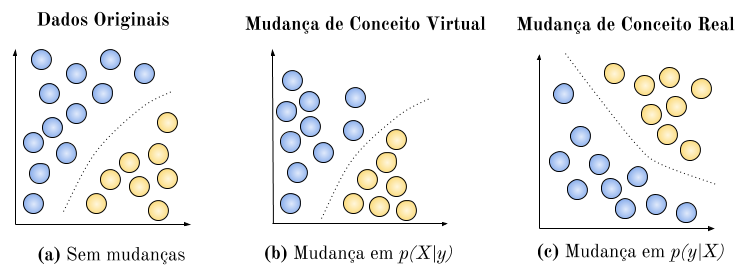
\includegraphics[scale=0.8]{imagens/concept_drift.png}
    \caption{Mudança de Conceito Virtual vs. Mudança de Conceito Real}
    \label{fig:real_and_virtual_concept_drift}
\end{center}
\end{figure}

Conforme \citeonline{Zliobaite:2010}, as mudanças de conceito podem ocorrer de forma abrupta, gradual, incremental ou recorrente.
A Figura \ref{fig:concept_drift_patterns} ilustra estes padrões, 
utilizando círculos na cor azul para representar o conceito \textit{A} e círculos na cor bege para o conceito \textit{B}:

\begin{figure}[H]
\begin{center}
    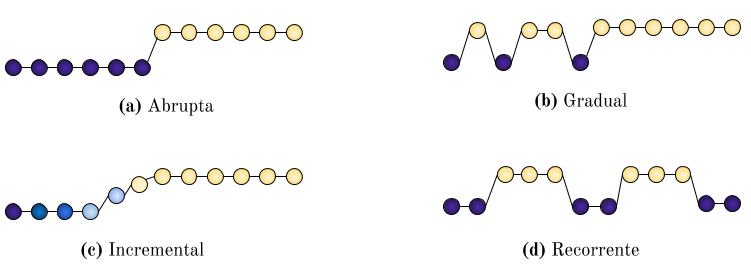
\includegraphics[scale=0.8]{imagens/concept_drift_patterns.png}
    \caption{Padrões de ocorrência de Mudanças de Conceito}
    \label{fig:concept_drift_patterns}
\end{center}
\end{figure}

Na mudança abrupta, o conceito \textit{A} é repentinamente substituído pelo conceito \textit{B} (Figura \ref{fig:concept_drift_patterns} (a)).

Na mudança gradual, ocorre uma transição mais suave entre os conceitos \textit{A} e \textit{B}.
Inicialmente, eventos pertencentes a ambos os conceitos coexistem.
Com o passar do tempo, os eventos pertencentes ao conceito \textit{A} diminuem de frequência, até pararem de ocorrer.
Por fim, os eventos pertencentes a \textit{B} se tornam predominantes (Figura \ref{fig:concept_drift_patterns} (b)).

A mudança incremental descreve a evolução de um único conceito ao longo do tempo.
Essa evolução pode ser discretizada como uma sequência de conceitos consecutivos.
Nesta sequência, cada conceito intermediário difere pouco dos seus conceitos antecessor e sucessor.
Portanto, as mudanças são notáveis apenas à longo prazo (Figura \ref{fig:concept_drift_patterns} (c)).

A mudança recorrente acontece quando um conceito anteriormente ativo reaparece após um determinado período de tempo. 
Contudo, não se trata de uma sazonalidade periódica, pois não é evidente o momento no qual o conceito voltará a ser ativo (Figura \ref{fig:concept_drift_patterns} (d)).

Este trabalho de mestrado propõe um método baseado em redes de função de base radial para detecção de mudanças de conceito reais em fluxos contínuos de dados, independente do padrão de ocorrência.
Na próxima subseção, será apresentada a terminologia do fenômeno mudança de conceito.

\subsection{Terminologia}

O fenômeno mudança de conceito tem sido estudado em diferentes comunidades de pesquisa, incluindo mineração de dados, 
aprendizado de máquina, estatística e recuperação de informação \cite{Zliobaite:2010}.
Contudo, o mesmo conceito pode ter diferentes nomeclaturas em cada comunidade.
Na Tabela \ref{tbl:taxonomy} são listados os termos correspondentes a mudança de conceito em cada área de pesquisa.

\begin{center} 
\begin{table}[H]
\label{tbl:taxonomy}
\begin{tabularx}{\textwidth}{|l|X|}
\cline{1-2}
\multicolumn{1}{|c|}{\textbf{Área}} & \multicolumn{1}{c|}{\textbf{Termos}}       \\ \cline{1-2}
Mineração de Dados                  & Mudança de Conceito                        \\ \cline{1-2}
Aprendizado de Máquina              & Mudança de Conceito, Mudança de Covariável \\ \cline{1-2}
Computação Evolucionária            & Ambiente Evolutivo, Ambiente em Mudança    \\ \cline{1-2}
IA e Robótica                       & Ambiente Dinâmico                          \\ \cline{1-2}
Estatísticas, Séries Temporais      & Não Estacionário                           \\ \cline{1-2}
Recuperação de Informação           & Evolução Temporal                          \\ \cline{1-2}
\end{tabularx}
\caption{Terminologia - Mudança de Conceito \cite{Zliobaite:2010}}
\end{table}
\end{center}

Outra fonte comum de equívocos são os termos detecção de \textit{outliers}, detecção de novidade, detecção de \textit{change points} e detecção de mudança de conceito.
Estes termos são muitas vezes utilizados de forma indistinta, mas, para o contexto deste trabalho, é importante distingui-los.

As técnicas para detecção de \textit{outliers} têm como objetivo identificar padrões de dados em desacordo com o comportamento esperado. Estes padrões são geralmente classificados como anomalias ou ruídos \cite{Chandola:2009:ADS:1541880.1541882}.

Os métodos para detecção de novidade identificam padrões ainda não observados, mas que se enquadram no comportamento esperado.
Estes métodos se diferenciam das técnicas para detecção de \textit{outliers} pois os novos padrões são incorporados ao modelo \cite{Chandola:2009:ADS:1541880.1541882}.

As estratégias para detecção de \textit{change points} identificam variações abruptas de valor, que podem representar transições entre estados, em séries temporais unidimensionais estacionárias \cite{Aminikhanghahi:2017:SMT:3086013.3086037}.

Por fim, os métodos para detecção de mudanças de conceito monitoram a distribuição dos dados ou indicadores (por exemplo: taxa de erro) das técnicas de aprendizado aplicadas, a fim de identificar a ocorrência de mudanças de conceito \cite{Gama:2014:SCD:2597757.2523813}.

Na próxima subseção, os principais algoritmos para detecção de mudança de conceito serão descritos.

\subsection{Algoritmos para Detecção de Mudança de Conceito}

Os algoritmos para detecção de mudança de conceito caracterizam e quantificam as mudanças de conceito através da delimitação dos instantes ou intervalos de tempo em que as mudanças ocorrem \cite{Basseville:1993:DAC:151741}.

Esses algoritmos se dividem em duas categorias, conforme a necessidade de rotulação dos dados \cite{Zliobaite:2010}:

\begin{description}
    \item[Algoritmos Explícitos/Supervisionados] Dependem da rotulação dos dados por um especialista.
    Estes rótulos são utilizados no cálculo de medidas de performance como taxa de erro e acurácia, que são monitoradas ao longo do tempo.
    Mudanças de conceito são sinalizadas quando essas medidas atingem um limite previamente definido.

    \item[Algoritmos Implícitos/Não Supervisionados] Independem da rotulação por especialistas, 
    baseando-se em características dos próprios dados ou indicadores das técnicas de aprendizado aplicadas.
    São mais propensos a alarmes falsos, mas essa independência os torna interessantes para contextos onde a obtenção de rótulos é dispendiosa, demorada ou inviável.
\end{description}

Segundo \citeonline{Gama:2014:SCD:2597757.2523813}, os algoritmos \textit{explícitos / supervisionados} podem ser segmentados em três subcategorias:

\begin{description}
    \item[Métodos Baseados em Análise Sequencial] Avaliam continuamente os indicadores de performance (por exemplo: taxa de erro) do classificador aplicado.
    A mudança de conceito é detectada quando esses indicadores atingem um limite pré-definido.
    Os algoritmos \textit{Cumulative Sum (CUSUM)}, \textit{PageHinkley (PH)} \cite{Page:CUSUM:PageHinkley:1954} e \textit{Geometric Moving Average (GMA)} \cite{Roberts:2000:CCT:338441.338464}
    são representantes desta subcategoria.

    \item[Abordagens baseadas em Estatística] Identificam mudanças de conceito através da análise de parâmetros estatísticos como média e desvio padrão associados aos resultados das predições.
    Os métodos \textit{Drift Detection Method (DDM)} \cite{GamaMCR04}, 
    \textit{Early Drift Detection Method (EDDM)} \cite{EDDM}, 
    \textit{Exponentially Weighted Moving Average (EWMA)} \cite{Ross:2012:EWM:2076039.2076307} e 
    \textit{Reactive Drift Detection Method (RDDM)} \cite{Barros:RDDM:2017} são exemplos desta subcategoria.

    \item[Métodos baseados em Janelas] Utilizam uma janela de tamanho fixo para sumarizar informações passadas e uma janela deslizante para sumarizar os dados recentes.
    Uma diferença significativa entre as distribuições dessas janelas implica na ocorrência de mudança de conceito.
    Esta diferença é verificada a partir de testes estatísticos ou desigualdades matemáticas, considerando como hipótese nula a igualdade das distribuições.
    Os algoritmos 
    \textit{Adaptive Windowing (ADWIN)} \cite{BifetG07}, 
    \textit{SeqDrift} \cite{PearsSK14:SeqDrift:2014}, 
    \textit{HDDMA} e \textit{HDDMW} \cite{BlancoCRBDM15:HDDMA:HDDMW:2015}
    pertencem a esta subcategoria.
\end{description}

De forma similar, os algoritmos \textit{implícitos / não supervisionados} também foram divididos em três subcategorias \cite{GONCALVES20148144}:

\begin{description}
    \item[Detecção de Novidade / Métodos de Agrupamento] 
    Utilizam técnicas derivadas dos métodos de agrupamento e de detecção de \textit{outliers} para identificar padrões ainda não observados.
    A partir dessa identificação, são realizados cálculos de distância e/ou densidade para confirmar a ocorrência de mudança de conceito \cite{Ryu:Kantardzic:2012}.
    Os métodos 
    \textit{OLINDDA} \cite{Spinosa:2007:OCA:1244002.1244107},
    \textit{MINAS} \cite{Faria:2013:NDA:2480362.2480515},
    \textit{Woo} \cite{Ryu:Kantardzic:2012},
    \textit{DETECTNOD} \cite{Hashemi:Hayat:DETECTNOD:2010},
    \textit{ECSMiner} \cite{Masud:2011:CNC:1978259.1978529} e
    \textit{GC3} \cite{Sethi2016b:GC3} fazem parte desta subcategoria.
    
    \item[Monitoramento de distribuição multivariada]
    Monitoram diretamente a distribuição dos dados para cada atributo.
    A distribuição de um conjunto de treinamento é sumarizada e utilizada como referência.
    Esta referência é, então, comparada à distribuição dos dados do conjunto atual.
    Diferenças significativas entre esses conjuntos indicam a ocorrência de mudança de conceito.
    Os algoritmos
    \textit{CoC} \cite{Lee:Magoules:CoC:2012},
    \textit{HDDDM} \cite{Ditzler:Polikar:HDDDM:2011},
    \textit{PCA-detect} \cite{Kuncheva:PCADetect:20085}
    são representantes desta subcategoria.

    \item[Monitoramento dependente de modelo]
    Dependem da aplicação de um algoritmo de classificação probabilístico, 
    pois as mudanças de conceito são detectadas a partir do monitoramento da probabilidade a posteriori calculada \cite{Zliobaite:2010}.
    Estes algoritmos conseguem reduzir a ocorrência de falsos positivos e tornar o processo computacionalmente eficiente, pois apenas um único fluxo univariado de valores é observado. 
    Os métodos 
    \textit{A-distance} \cite{Dredze:ADistance:2010585},
    \textit{CDBD} \cite{Lindstrom:CDBD:2013} e
    \textit{Margin} \cite{Dries:Margin:2009} integram esta subcategoria.
\end{description}

Por fim, a Tabela \ref{tbl:abordagens} sumariza as categorias, as subcategorias e as respectivas técnicas abordadas nesta seção.

\begin{table}[!ht]
    \centering
    \resizebox{\textwidth}{!}{%
    \begin{tabular}[t]{@{}lllll@{}}
    \hline \\
    Algoritmos Explícitos/Supervisionados     & Métodos Baseados em Análise Sequencial        & \begin{tabular}[t]{@{}l@{}} Cumulative Sum (CUSUM) \\ PageHinkley (PH) \cite{Page:CUSUM:PageHinkley:1954} \\ Geometric Moving Average (GMA) \cite{Roberts:2000:CCT:338441.338464}\end{tabular}                                                                                                                        &  &  \\ \\
                                              & Abordagens baseadas em Estatística            & \begin{tabular}[t]{@{}l@{}} Drift Detection Method (DDM) \cite{GamaMCR04} \\  Early Drift Detection Method (EDDM) \cite{EDDM} \\  Exponentially Weighted Moving Average (EWMA) \cite{Ross:2012:EWM:2076039.2076307} \\ Reactive Drift Detection Method (RDDM) \cite{Barros:RDDM:2017} \end{tabular}                                                                &  &  \\ \\
                                              & Métodos baseados em Janelas                   & \begin{tabular}[t]{@{}l@{}} Adaptive Windowing (ADWIN) \cite{BifetG07} \\   SeqDrift \cite{PearsSK14:SeqDrift:2014} \\   HDDMA/HDDMW \cite{BlancoCRBDM15:HDDMA:HDDMW:2015} \end{tabular}                                                                                            &  &  \\ \\
    
    Algoritmos Implícitos/Não Supervisionados & Detecção de Novidade / Métodos de Agrupamento & \begin{tabular}[t]{@{}l@{}} OLINDDA \cite{Spinosa:2007:OCA:1244002.1244107} \\   MINAS \cite{Faria:2013:NDA:2480362.2480515} \\   Woo \cite{Ryu:Kantardzic:2012} \\   DETECTNOD \cite{Hashemi:Hayat:DETECTNOD:2010} \\   ECSMiner \cite{Masud:2011:CNC:1978259.1978529} \\   GC3 \cite{Sethi2016b:GC3} \end{tabular} &  &  \\ \\
                                              & Monitoramento de distribuição multivariada    & \begin{tabular}[t]{@{}l@{}} CoC \cite{Lee:Magoules:CoC:2012} \\ HDDDM \cite{Ditzler:Polikar:HDDDM:2011} \\ PCA-detect \cite{Kuncheva:PCADetect:20085} \end{tabular}                                       &  &  \\ \\
                                              & Monitoramento dependente de modelo            & \begin{tabular}[t]{@{}l@{}} A-distance \cite{Dredze:ADistance:2010585} \\ CDBD \cite{Lindstrom:CDBD:2013} \\ Margin \cite{Dries:Margin:2009} \end{tabular}                                                                                        &  &  \\ \\
    \hline
    \end{tabular}%
    }
    \caption{Sumário - Algoritmos para Detecçaõ de Mudanças de Conceito \cite{Sethi:2017:RDC:3096751.3096864}}
    \label{tbl:abordagens}
\end{table}

O método de detecção proposto neste trabalho se enquadra na categoria de algoritmos \textit{implícitos / não supervisionados}, mais especificamente na subcategoria \textit{detecção de novidades / métodos de agrupamento}.
Na próxima seção, as ferramentas utilizadas para implementação e validação deste método serão apresentadas.

\subsection{Ferramentas}

Nesta seção, os frameworks \textit{Massive Online Analysis} (MOA) e \textit{Tornado} serão apresentados.
Estas ferramentas permitem a implementação e a validação de novas técnicas de detecção de mudanças de conceito.
Além de possibilitarem a comparação com o estado da arte, pois dispõem de um vasto conjunto de algoritmos já implementados.
Ambas as ferramentas foram utilizadas durante o desenvolvimento deste projeto de trabalho de mestrado.

\subsection{MOA}

Atualmente, o \textit{MOA – Massive Online Analysis}\footnote{https://moa.cms.waikato.ac.nz/} é o principal framework para mineração de dados em fluxos contínuos \cite{Bifet:2010:MMO:1756006.1859903}.
O projeto é de código-aberto\footnote{https://github.com/Waikato/moa} e apresenta uma comunidade bastante ativa e crescente.
A aplicação é composta por uma ampla coleção de algoritmos da área de aprendizado de máquina, contemplando técnicas de classificação, regressão, agrupamento, busca por padrões, detecção de \textit{outliers}, detecção de mudanças de conceito e sistemas de recomendação.
Além das implementações, também estão disponíveis rotinas para avaliação dessas técnicas.
A aplicação é desenvolvida em Java, o que permite a sua execução nos principais sistemas operacionais e a integração com o projeto WEKA \cite{Hall:2009:WDM:1656274.1656278}.

O MOA divide as suas funcionalidades em tarefas (\textit{tasks}).
Estas tarefas podem ser executadas a partir da interface gráfica (GUI) ou por linha de comando.
A interface gráfica permite executar múltiplas tarefas de forma concorrente, 
controlar suas execuções e visualizar os resultados parciais.
A tela principal da aplicação é demonstrada na Figura \ref{fig:moa}.

\begin{figure}[H]
\begin{center}
    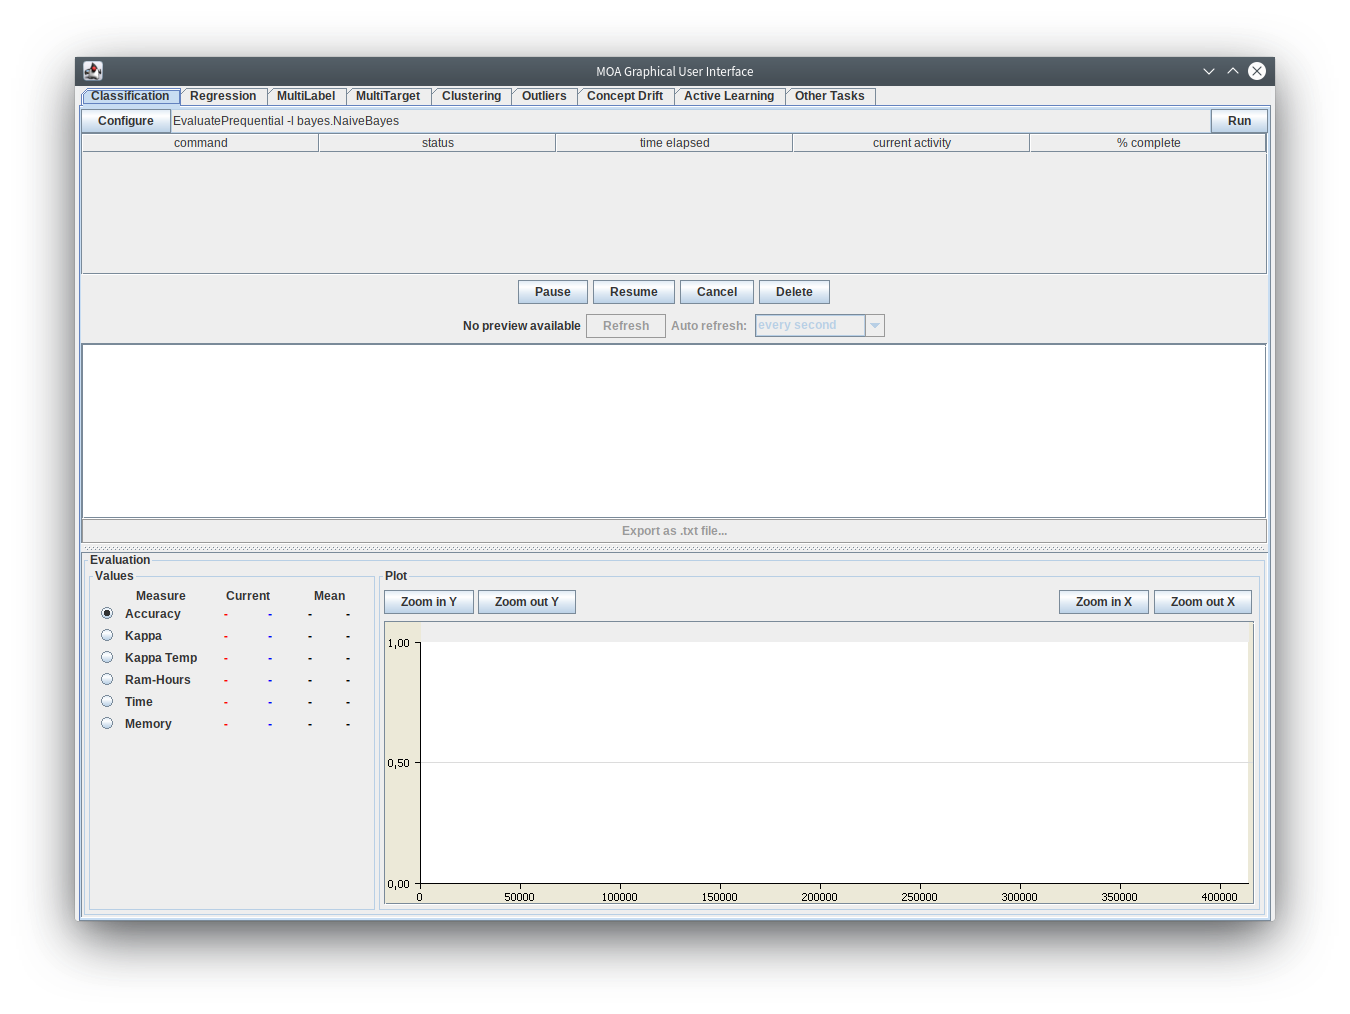
\includegraphics[scale=0.4]{imagens/moa.png}
    \caption{MOA - Tela Inicial}
    \label{fig:moa}
\end{center}
\end{figure}

A aplicação é capaz de ler arquivos em formato \textit{ARFF}, popularizados pelo projeto WEKA.
A ferramenta também permite a produção de fluxos de dados dinamicamente, através de geradores.
Alguns dos geradores de fluxo disponíveis no MOA são:
\textit{Random Trees} \cite{Domingos:2000:MHD:347090.347107}
\textit{SEA} \cite{Street:2001:SEA:502512.502568}, 
\textit{STAGGER} \cite{Schlimmer1986}, 
\textit{Rotating Hyperplane} \cite{Wang:2003:MCD:956750.956778},
\textit{Random RBF}, 
\textit{LED} \cite{Gama:2003:ADT:956750.956813}, 
\textit{Waveform} \cite{Gama:2003:ADT:956750.956813}, 
 e \textit{Function} \cite{Jin:2003:EDT:956750.956821}.

Outra funcionalidade importante do framework é a possibilidade de adicionar mudanças de conceito a fluxos estacionários existentes.
Esse processo é realizado através de uma função sigmóide, que modela o evento de mudança de conceito como uma combinação balanceada de duas distribuições homogêneas, 
que caracterizam os conceitos-alvo antes e depois da mudança.
Além destes conceitos, o usuário também pode definir o momento da mudança e a sua duração \cite{Bifet:2010:MMO:1756006.1859903}.

Os principais métodos para detecção de mudança de conceito propostos na literatura estão disponíveis no MOA.
Além disso, a arquitetura do framework é modular, permitindo a implementação de novos detectores de forma trivial.
Por exemplo, para criar um novo detector, basta estender a classe abstrata \texttt{AbstractChangeDetector} e implementar o algoritmo desejado.
A janela de configuração deste detector, similar a Figura \ref{fig:moa_detector}, será criada dinamicamente, a partir dos atributos definidos na classe.

\begin{figure}[H]
\begin{center}
    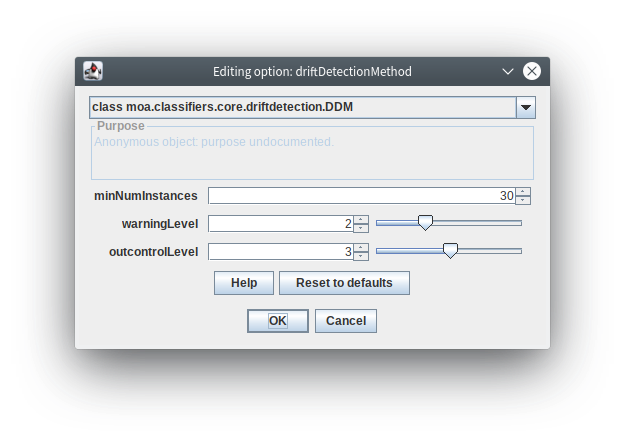
\includegraphics[scale=1]{imagens/detector.png}
    \caption{MOA - Configuração detector}
    \label{fig:moa_detector}
\end{center}
\end{figure}
    

O MOA dispõe de diversas classes para avaliação de técnicas de aprendizado de máquina. 
Para este trabalho, destacam-se as classes \texttt{DriftDetectionMethodClassifier} e \texttt{BasicConceptDriftPerformanceEvaluator}, 
que realizam a análise de algoritmos para detecção de mudança de conceito.
A classe \texttt{DriftDetectionMethodClassifier} permite avaliar técnicas de detecção que encapsulam um classificador.
Por sua vez, a classe \texttt{BasicConceptDriftPerformanceEvaluator} avalia a performance das técnicas de detecção que atuam diretamente sobre o fluxo de dados, sem utilizarem um algoritmo de classificação.
Estes avaliadores e os seus indicadores serão detalhados juntamente com os resultados dos experimentos iniciais, no Capítulo \ref{experimentos_iniciais}.

\subsection{Tornado}

O \textit{Tornado} é um framework para avaliação de algoritmos de detecção de mudança de conceito \cite{Pesaranghader:Tornado}.
O projeto é desenvolvido na linguagem Python e o seu código está disponível\footnote{https://github.com/alipsgh/tornado}.
O framework se diferencia do \textit{MOA} por apresentar um cenário de avaliação específico: 
analisar a execução, em paralelo, de pares (classificador, detector de mudança de conceito), 
para identificar o par ótimo ao longo do tempo, em relação ao fluxo de dados.

\begin{figure}[H]
\begin{center}
    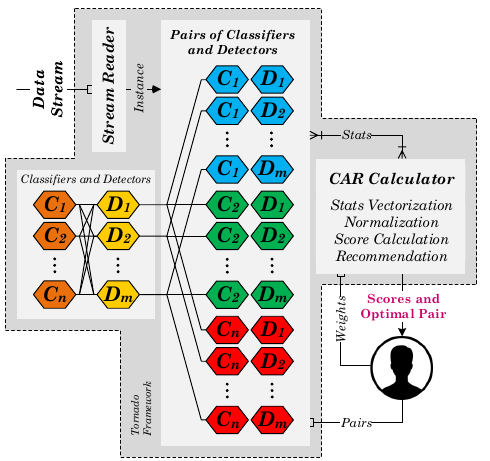
\includegraphics[scale=0.75]{imagens/tornado.png}
    \caption{Framework Tornado \cite{Pesaranghader:Tornado}.}
    \label{fig:tornado}
\end{center}
\end{figure}

Conforme apresentado na Figura \ref{fig:tornado}, os principais componentes do framework são: 
\textit{Stream Reader}, \textit{Classifiers}, \textit{Detectors}, \textit{Classifier-Detector Pairs} e \textit{CAR Calculator}.
A entrada de dados é composta por um fluxo (\textit{Stream}), uma lista de pares (classificador, detector) e um vetor com pesos.

O componente \textit{Stream Reader} recepciona as instâncias e as encaminha para construção do modelo de forma incremental. 
Por seguir a abordagem \textit{prequential}, cada instância é primeiramente utilizada para testes e depois como treinamento.
Simultaneamente, os classificadores enviam suas estatísticas aos detectores, para que a mudança de conceito possa ser sinalizada.
Por fim, o componente \textit{CAR Calculator} calcula uma pontuação para cada par (classificador e detector), considerando taxa de erro, atraso para detecção da mudança de conceito, falsos positivos, falsos negativos, quantidade de memória utilizada e tempo de execução \cite{Pesaranghader:Tornado}.

O framework apresenta ao usuário o par ótimo para cada instante da execução. 
A abordagem de avaliação adotada pelo framework é relevante, pois este par pode mudar ao longo do tempo, devido ao aprendizado incremental ou às mudanças de conceito.
A Figura \ref{fig:tornado_out2} apresenta um exemplo de resultado produzido pela ferramenta.

\begin{figure}[H]
\begin{center}
    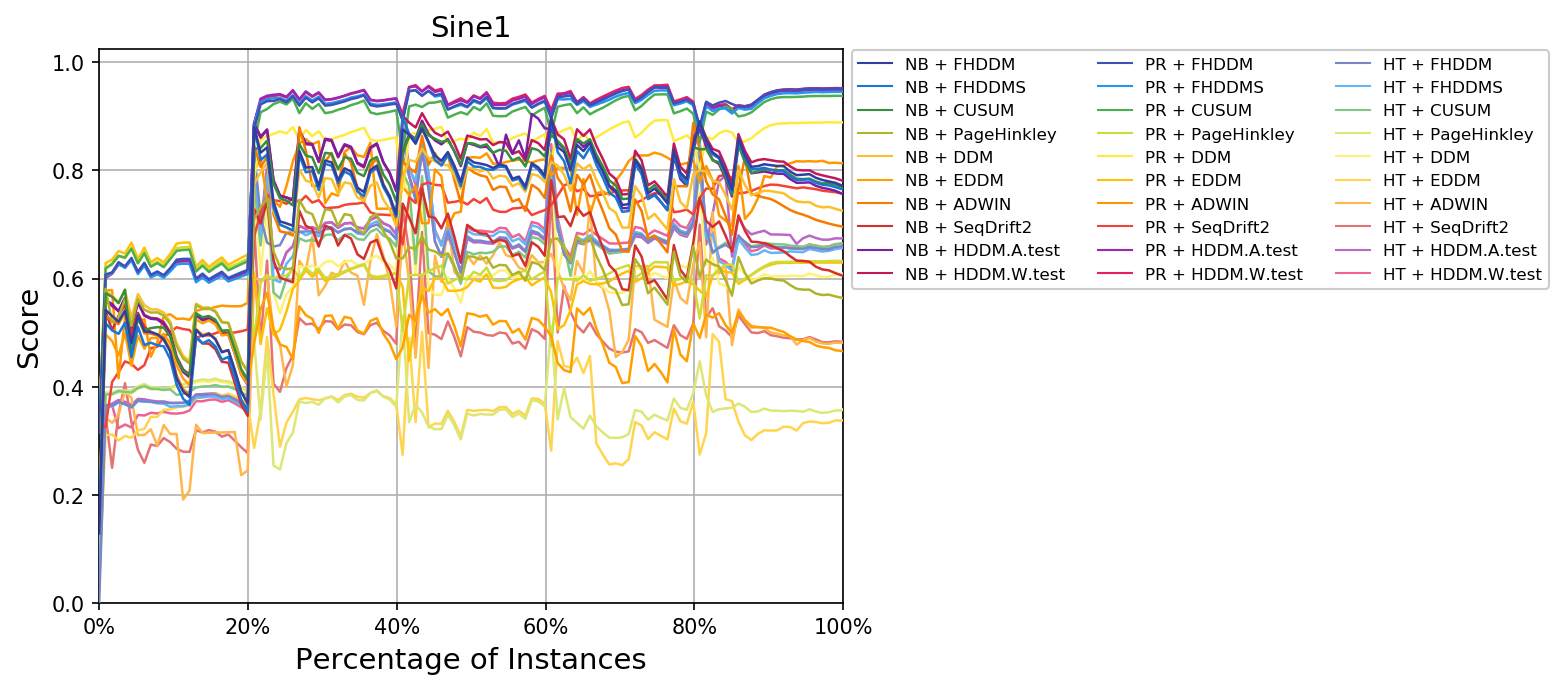
\includegraphics[scale=0.6]{imagens/tornado_out2.png}
    \caption{Tornado - Resultado para múltiplos pares \cite{Pesaranghader:Tornado}}
    \label{fig:tornado_out2}
\end{center}
\end{figure}

Neste trabalho, o algoritmo proposto foi implementado e testado nas duas ferramentas apresentadas.
Os detalhes de implementação e os resultados desses testes serão discutidos no Capítulo \ref{experimentos_iniciais}.
A seguir, as redes de função de base radial são detalhadas.

\section{Redes de Função de Base Radial}


Uma Rede de Função de Base Radial (\textit{radial basis function, RBF,} em inglês) pode ser definida como um modelo de múltiplas camadas alimentadas adiante (\textit{feedforward}), 
capaz de analisar padrões complexos e resolver problemas não-linearmente separáveis, utilizando uma abordagem de aproximação de funções.
Estas redes têm como principal diferencial a sua forma de ativação, realizada através do cálculo da distância entre o dado e um centro definido \cite{Braga:RedesNeuraisTeoriaAplicacoes}.

A arquitetura de uma rede de função de base radial, em sua forma mais básica, envolve três camadas.
A camada de entrada contém nós de fonte (unidades sensoriais) que conectam a rede ao seu ambiente.
A camada intermediária, única camada oculta da rede, 
utiliza funções de base radial para realizar uma transformação não-linear dos dados de entrada para um espaço de alta dimensionalidade.
Por fim, a camada de saída, através de uma combinação linear, fornece a resposta da rede ao padrão (sinal) de ativação aplicado à camada de entrada \cite{Rojas:1996:NNS:235222}. 
A Figura \ref{fig:rbg_arq} demonstra essa arquitetura.

\begin{figure}[H]
\begin{center}
    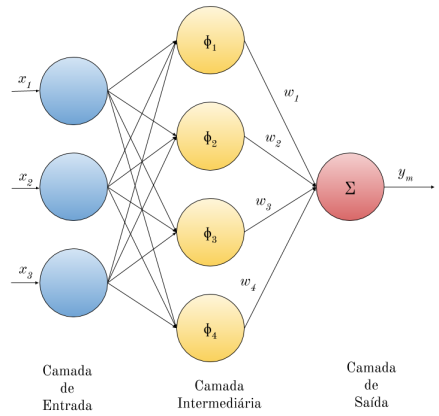
\includegraphics[scale=1]{imagens/rbf_arq.png}
    \caption{Arquitetura RBF}
    \label{fig:rbg_arq}
\end{center}
\end{figure}

A transformação não-linear dos dados de entrada para um espaço de alta dimensionalidade é justificada matematicamente pelo teorema de \citeonline{cover1965browse}, 
segundo o qual, ``um problema complexo de classificação de padrões disposto não linearmente em um espaço de alta dimensionalidade tem maior probabilidade de ser linearmente separável do que em um espaço de baixa dimensionalidade''.

Essa transformação é realizada por funções de base radial presentes na camada intermediária. 
Na literatura, uma das funções mais utilizadas para esta tarefa é a função gaussiana, representada na Equação \ref{eq:gaussiana}:

\begin{equation} \label{eq:gaussiana}
    \phi (v_{i})=\exp \left(-{\frac  {\|v_{i}-c_{i}\|^{2}}{2\sigma ^{2}}}\right)
\end{equation}

onde, $v$ é o valor de entrada, $c_i$ representa o centro e $\sigma$ é o parâmetro limitador do raio.
Assim, a classificação realizada por uma rede de função de base radial consiste na resolução das funções \ref{eq:rbf1} e \ref{eq:rbf2}:

\begin{equation} \label{eq:rbf1}
    f(x)=\sum _{{i=1}}^{N}w_{ij}\varphi (||{\mathbf  {x}}-{\mathbf  {t}}_{i}||)
\end{equation}

\begin{equation} \label{eq:rbf2}
    y_i=\sum _{{i=1}}^{N}w_{ij}\phi (||{\mathbf  {x}}-{\mathbf  {t}}_{i}||) + w_{j_0}
\end{equation}

A resolução dessas equações produz o sistema responsável por produzir o resultado final da rede (Equação \ref{eq:rbf3}):

\begin{equation} \label{eq:rbf3}
\begin{bmatrix}
    \varphi (||{{x_1}}-{{t}}_{1}||) & \varphi (||{{x_1}}-{{t}}_{2}||) & \dots & \varphi (||{{x_1}}-{{t}}_{N}||) \\
    \varphi (||{{x_2}}-{{t}}_{1}||) & \varphi (||{{x_2}}-{{t}}_{2}||) & \dots & \varphi (||{{x_2}}-{{t}}_{N}||) \\
    \hdotsfor{5} \\
    \varphi (||{{x_N}}-{{t}}_{1}||) & \varphi (||{{x_N}}-{{t}}_{2}||) & \dots & \varphi (||{{x_N}}-{{t}}_{N}||)
\end{bmatrix}
\begin{bmatrix}
    w_1 \\
    w_2 \\
    \vdots \\
    w_N \\
\end{bmatrix}
=
\begin{bmatrix}
    y_1 \\
    y_2 \\
    \vdots \\
    y_N \\
\end{bmatrix}
\end{equation}

onde $w_{ij}$ são os pesos de cada conexão, $\phi$ é a matriz de interpolação originada do conjunto de $N$ funções
de base radial aplicadas nas entradas $x$ e dos seus respectivos centros $t_i$,
$w_{j_0}$ representa o bias, $\varphi (||{{x}}-{{t}}_{i}||)$ é o conjunto de $N$ funções de base radial,
$||\ldots||$ é a norma euclidiana e $y$ são as saídas geradas pela rede.

O algoritmo proposto neste trabalho utiliza as camadas inicial e intermediária das redes de função de base radial para compôr um novo método de detecção de mudanças de conceito.
A camada intermediária cria, de forma implícita, agrupamentos no espaço oculto de alta dimensionalidade.
Portanto, é possível utilizar a criação de novos centros e a mudança do centro ativo como indicadores de possíveis mudanças de conceito.
A técnica desenvolvida será discutida em detalhes no Capítulo \ref{plano_pesquisa}.

Na próxima seção, os trabalhos relacionados encontrados na literatura são apresentados.

\section{Trabalhos Relacionados}

Além das referências básicas apresentadas neste capítulo, foi realizada uma pesquisa na literatura visando identificar trabalhos 
que utilizam redes de função de base radial para identificação de mudanças de conceito ou para outras tarefas correlatas.

\citeonline{Jianping:Venkateswarlu:RBF:SpeakerIdentification} utilizaram redes de função de base radial em um novo método para detecção de novidades.
A técnica proposta atua sobre cenários estacionários e foi aplicada ao problema de identificação da fala.
Seu principal diferencial é a utilização do algoritmo \textit{k-means} para definir os centros e as matrizes de covariância da rede.

\citeonline{Roberts:Penny:Novelty:Confidence} propuseram um método para detecção de novidades baseado em um comitê de redes de função de base radial.
Novos padrões são detectados a partir do monitoramento das taxas de erro e confiança desse comitê.
A técnica proposta foi testada na classificação de pacientes com problemas de tremor muscular.

Por fim, \citeonline{Bazargani2018RadialBF} utilizaram redes RBF para detecção de anomalias em fluxos de dados.
O método proposto modifica às funções de perda (\textit{loss}), transformando as redes de função de base radial em classificadores de classe única.
Essa alteração permitiu a identificação de exemplos divergentes dos padrões conhecidos.

\section{Considerações Finais}

Neste capítulo foram apresentados os principais conceitos utilizados neste projeto de trabalho de mestrado.
Foram discutidos conceitos de fluxos contínuos de dados, 
técnicas de aprendizado de máquina, 
mudanças de conceito,
técnicas de detecção de mudanças de conceito e redes de função de base radial.
Por fim, foram apresentados os trabalhos relacionados encontrados na literatura.
No próximo capítulo, o plano de pesquisa será detalhado.

\xchapter{Plano de Pesquisa}{} \label{plano_pesquisa}
\section{Considerações Iniciais}

Este capítulo descreve como a pesquisa proposta neste mestrado será desenvolvida.
O objetivo principal é a implementação de um algoritmo para detecção de mudanças de conceito em fluxos de dados contínuos utilizando as camadas inicial e intermediária das redes da função de base radial.
A seguir, são apresentados detalhes sobre cada etapa do desenvolvimento do projeto.

\section{Descrição do Problema}

A partir da Teoria Bayesiana de Decisão, apresentada na Seção \ref{sec:mudanca_de_conceito}, é possível afirmar que existe mudança de conceito entre os instantes $t_0$ e $t_1$ se:

\begin{equation} \label{eq:mudanca_de_conceito}
    {\exists}X : p_{t_0}(X, c) \ne p_{t_1}(X, c)
\end{equation}

onde $p_{t_0}$ e $p_{t_1}$ denotam as distribuições de probabilidades conjuntas nos instantes $t_0$ e $t_1$, respectivamente, 
para $X$ e $c$ \cite{Gama:2014:SCD:2597757.2523813}. 
Isto é, um conjunto de exemplos possui rótulos de classe legítimos em $t_0$, mas passa a ter rótulos diferentes, também legítimos, em $t_1$ \cite{Kolter:2007:DWM:1314498.1390333}.
Esta mudança pode ocorrer devido a alterações no contexto do processo gerador ou na distribuição dos dados, 
e pode impactar a acurácia de modelos de decisão utilizados.

Considerando que a camada intermediária (oculta) de uma rede de função de base radial realiza o agrupamento dos dados de entrada em clusters, 
transformando padrões de entrada não linearmente separáveis em um conjunto de valores linearmente separáveis \cite{Jianping:Venkateswarlu:RBF:SpeakerIdentification}, 
este projeto de mestrado tem como objetivo comprovar a hipótese que mudanças de conceito em fluxos contínuos de dados podem ser detectadas através de redes de função de base radial, de forma online e independente de exemplos prévios ou rótulos.

Para exemplificar a execução desta proposta de mestrado, considere o conjunto $D = \{0.1, 0.13, 0.14, 0.4, 0.5, 0.6, 0.16, 0.14\}$, recorte do fluxo contínuo utilizado como entrada.

% Assumindo que sejam produtos de um fluxo contínuo de dados, estes valores são passados para a camada de entrada da rede de função de base radial.
% Esta camada encaminha o valor para uma função de base radial Gaussiana (\ref{eq:gaussiana}). 



\section{Atividades de Pesquisa}
\blindtext

\section{Considerações Finais}
\blindtext

\xchapter{Experimentos Iniciais}{} \label{experimentos_iniciais}
\section{Considerações Iniciais}
\blindtext

\section{Configuração dos Experimentos}
\blindtext

\section{Método de Pettitt}
\blindtext

\section{Redes de Função de Base Radial}
\blindtext

\section{Considerações Finais}
\blindtext


%% Parte pos-textual
\backmatter

% Bibliografia
% É aconselhável utilizar o BibTeX a partir de um arquivo, digamos "biblio.bib".
% Para ajuda na criação do arquivo .bib e utilização do BibTeX, recorra ao
% BibTeXpress em www.cin.ufpe.br/~paguso/bibtexpress
\bibliographystyle{abntex2-alf}
\bibliography{biblio}

% Apendices
% Comente se naoo houver apendices
%\appendix

%\xchapter{Exemplo de Ap\^endice}{} %sem preambulo
%\lipsum
% Eh aconselhavel criar cada apendice em um arquivo separado, digamos
% "apendice1.tex", "apendice.tex", ... "apendiceM.tex" e depois
% inclui--los com:
%\xchapter{Decomposição das séries temporais}{} %sem preambulo
\label{apendice1}
\section{Considerações Iniciais}
Neste apêndice consta as 40 séries temporais utilizadas nos experimentos mostrados no Capitulo \ref{experimentos}. As séries foram divididas em 4 tipos conforme a Tabela \ref{series}, onde o tipo representa um conjunto de 10 séries senoide ou cossenoide, sendo acrescida de ruído ou acrescida de ruído e tendência.
Nas imagens são representadas, a séries original,   seu componente determinístico e seu componente estocástico, os quais foram extraídos após a decomposição.
\section{Séries TIPO 1}
10 séries cossenoide com ruído ao longo da série.
\graphicspath{{imagens/}}
\begin{figure}[H]
\begin{center}
  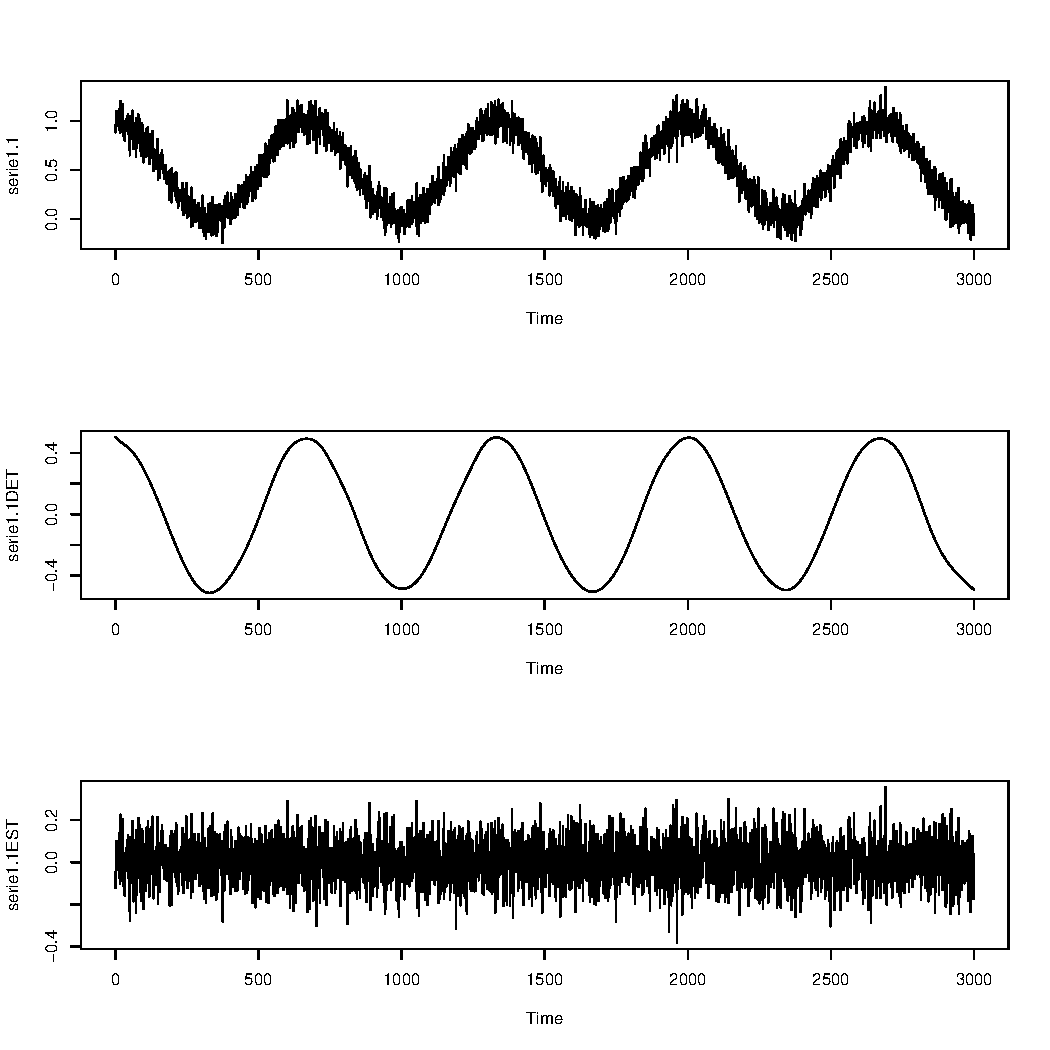
\includegraphics[scale=0.43]{serie1_1.pdf} \quad
  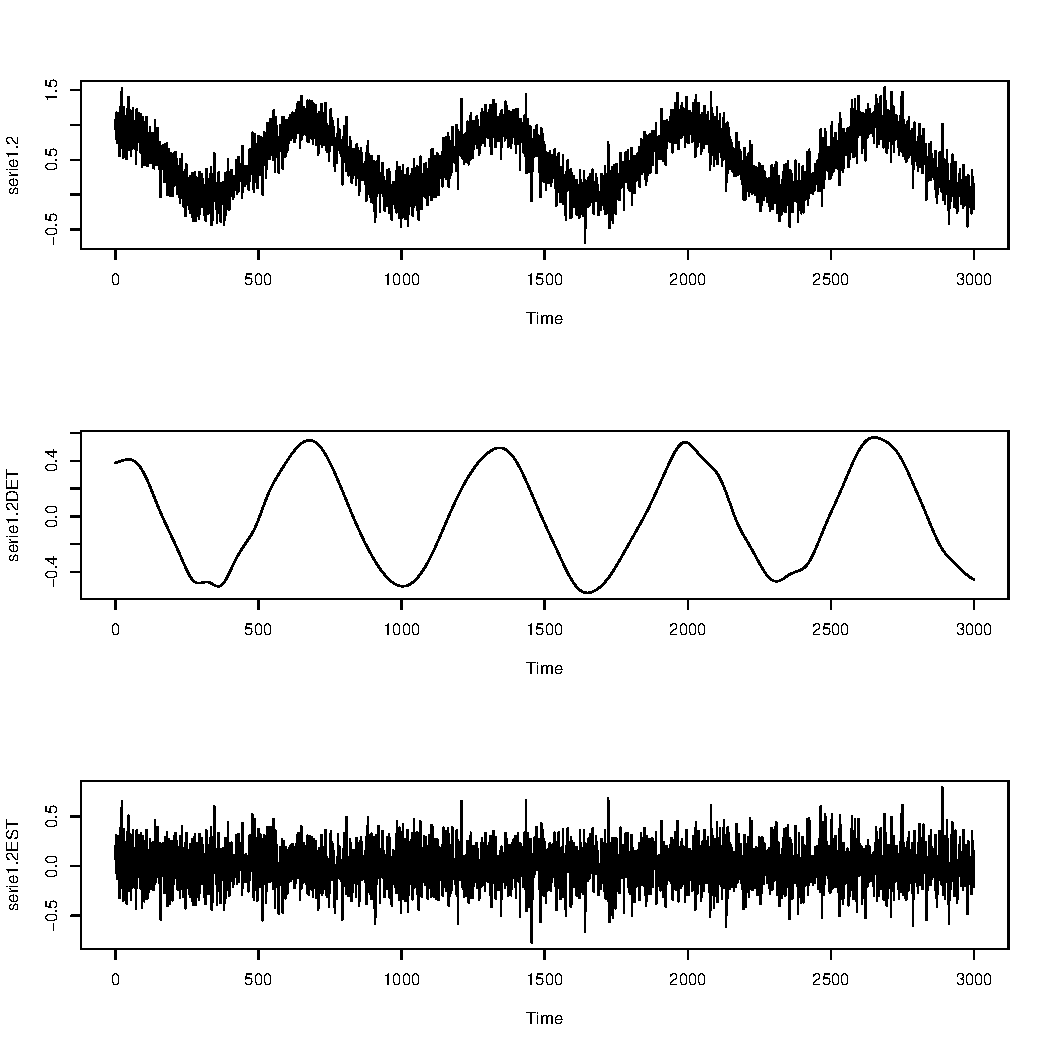
\includegraphics[scale=0.43]{serie1_2.pdf}
  \caption{Série 1.1 e Série 1.2}

\end{center}
\end{figure}

\graphicspath{{imagens/}}
\begin{figure}[H]
\begin{center}
  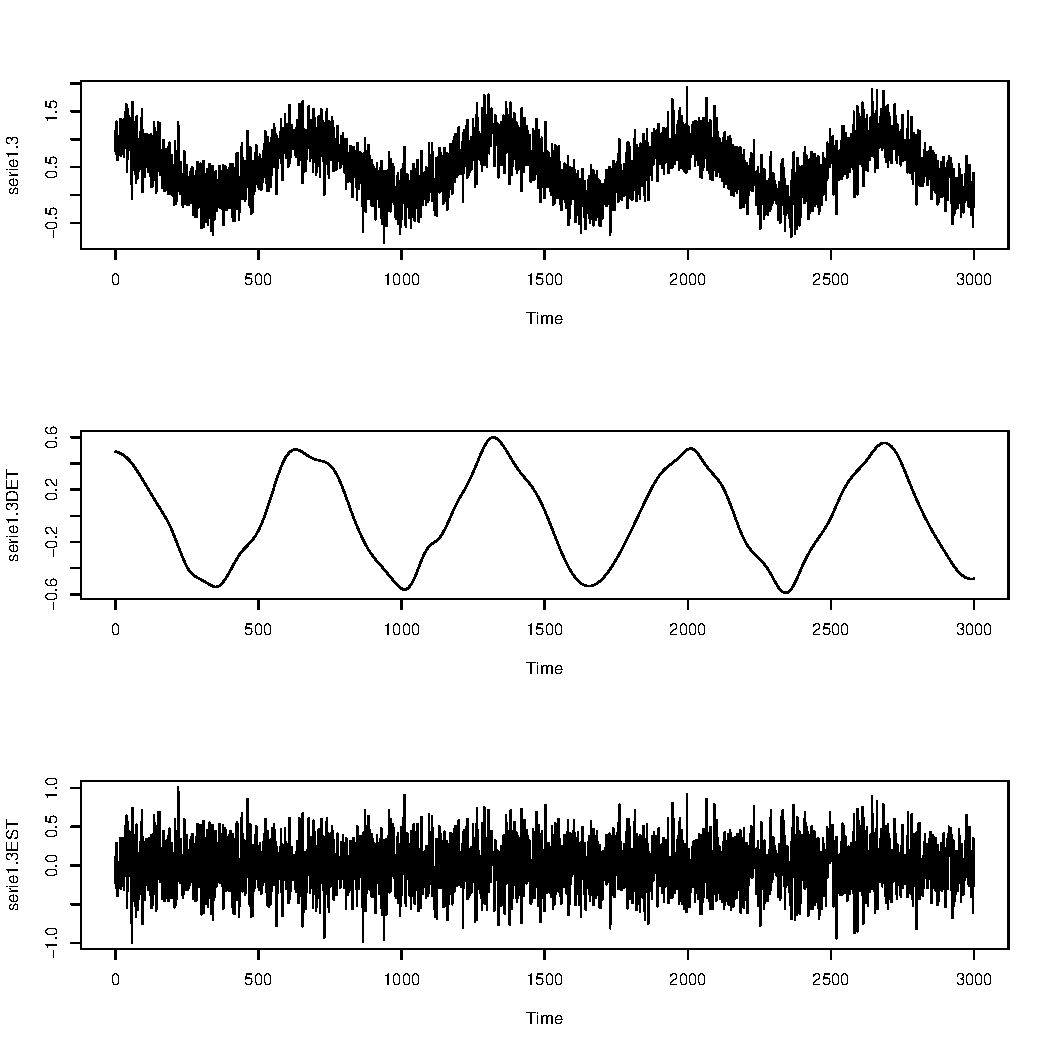
\includegraphics[scale=0.43]{serie1_3.pdf} \quad
  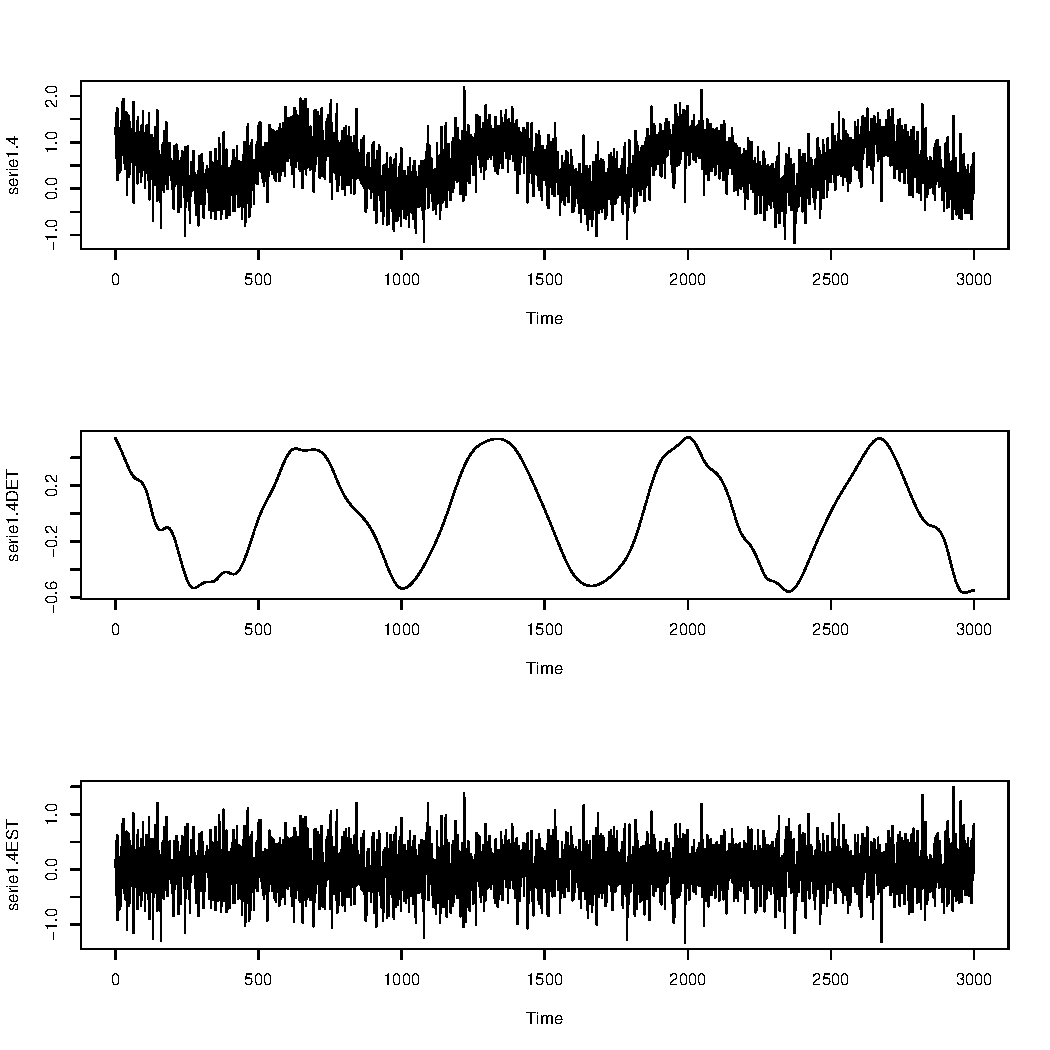
\includegraphics[scale=0.43]{serie1_4.pdf}
  \caption{Série 1.3 e Série 1.4}

\end{center}
\end{figure}

\graphicspath{{imagens/}}
\begin{figure}[H]
\begin{center}
  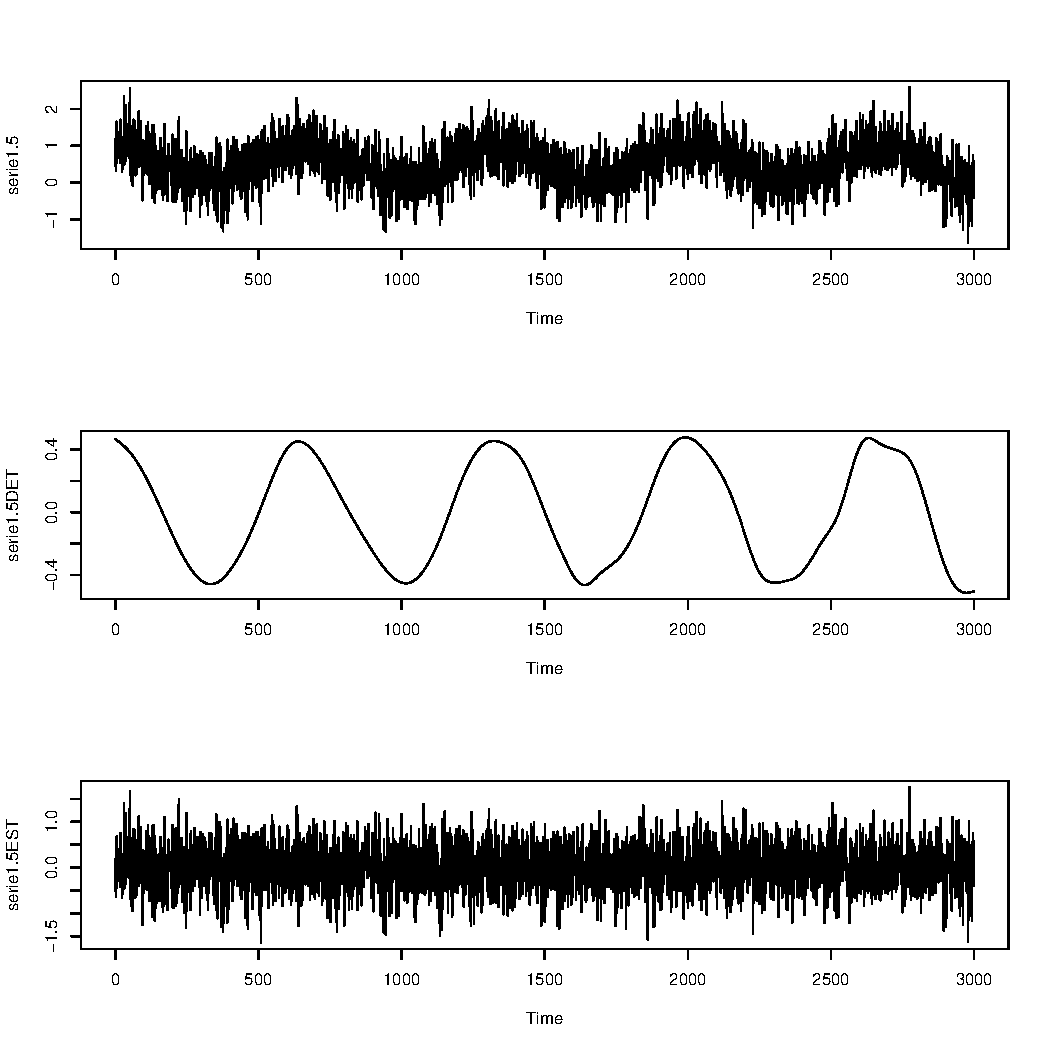
\includegraphics[scale=0.43]{serie1_5.pdf} \quad
  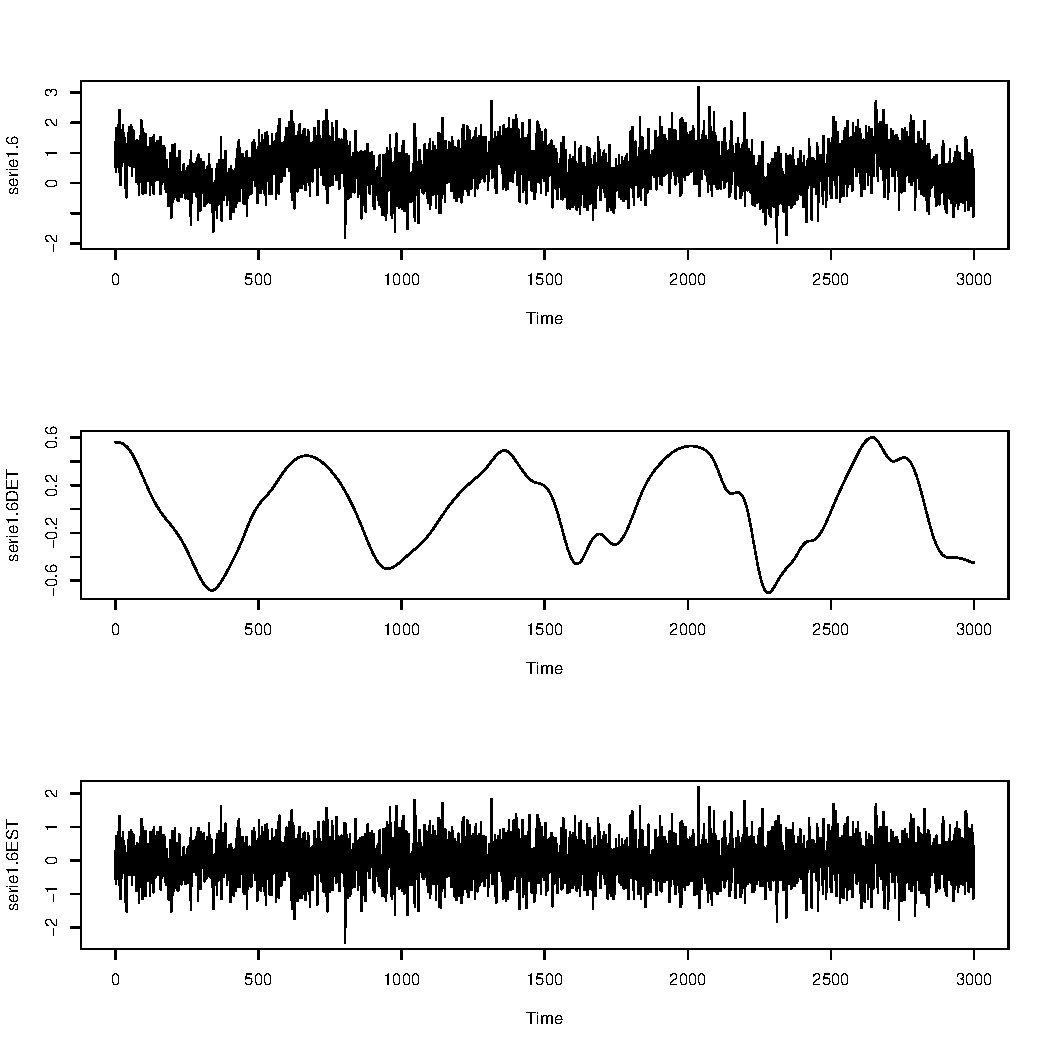
\includegraphics[scale=0.43]{serie1_6.pdf}
  \caption{Série 1.5 e Série 1.6}

\end{center}
\end{figure}

\graphicspath{{imagens/}}
\begin{figure}[H]
\begin{center}
  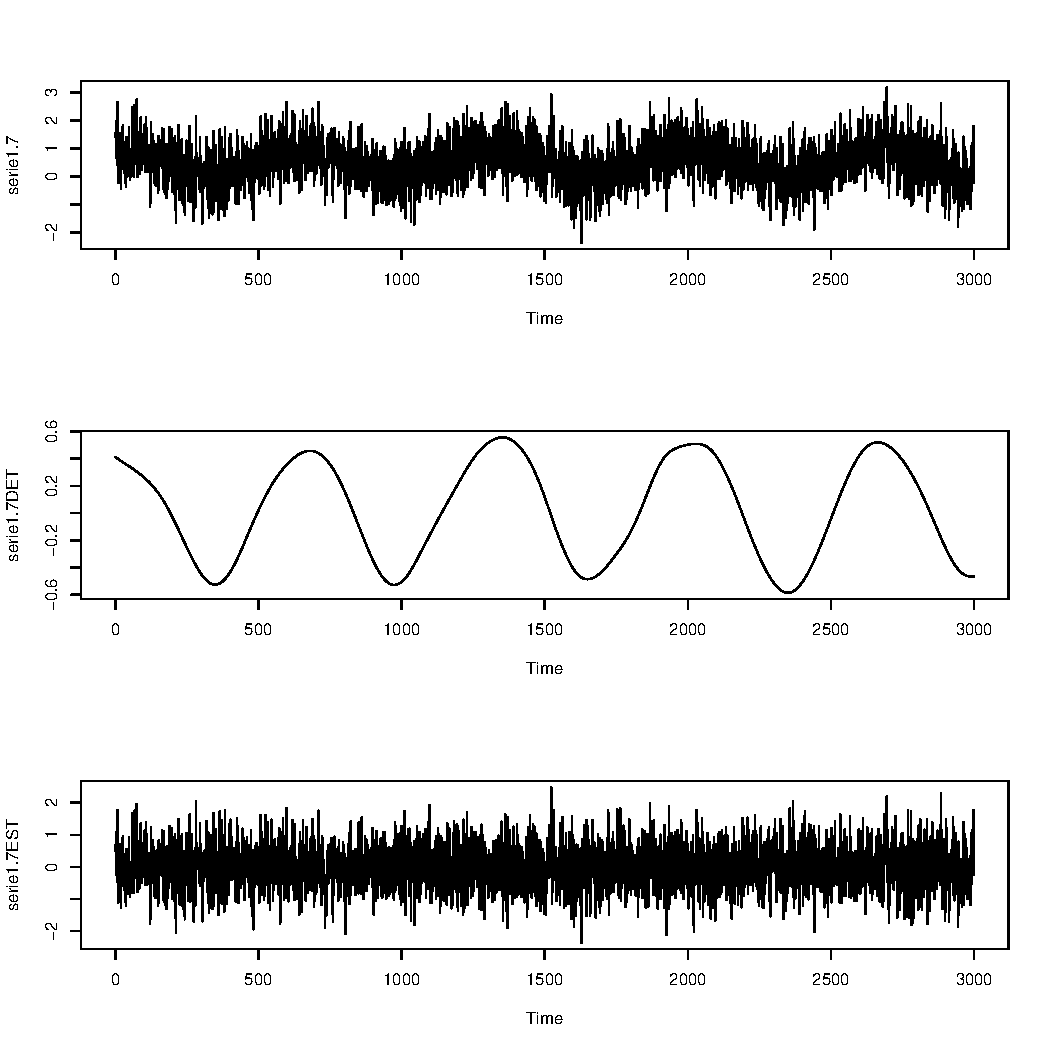
\includegraphics[scale=0.43]{serie1_7.pdf} \quad
  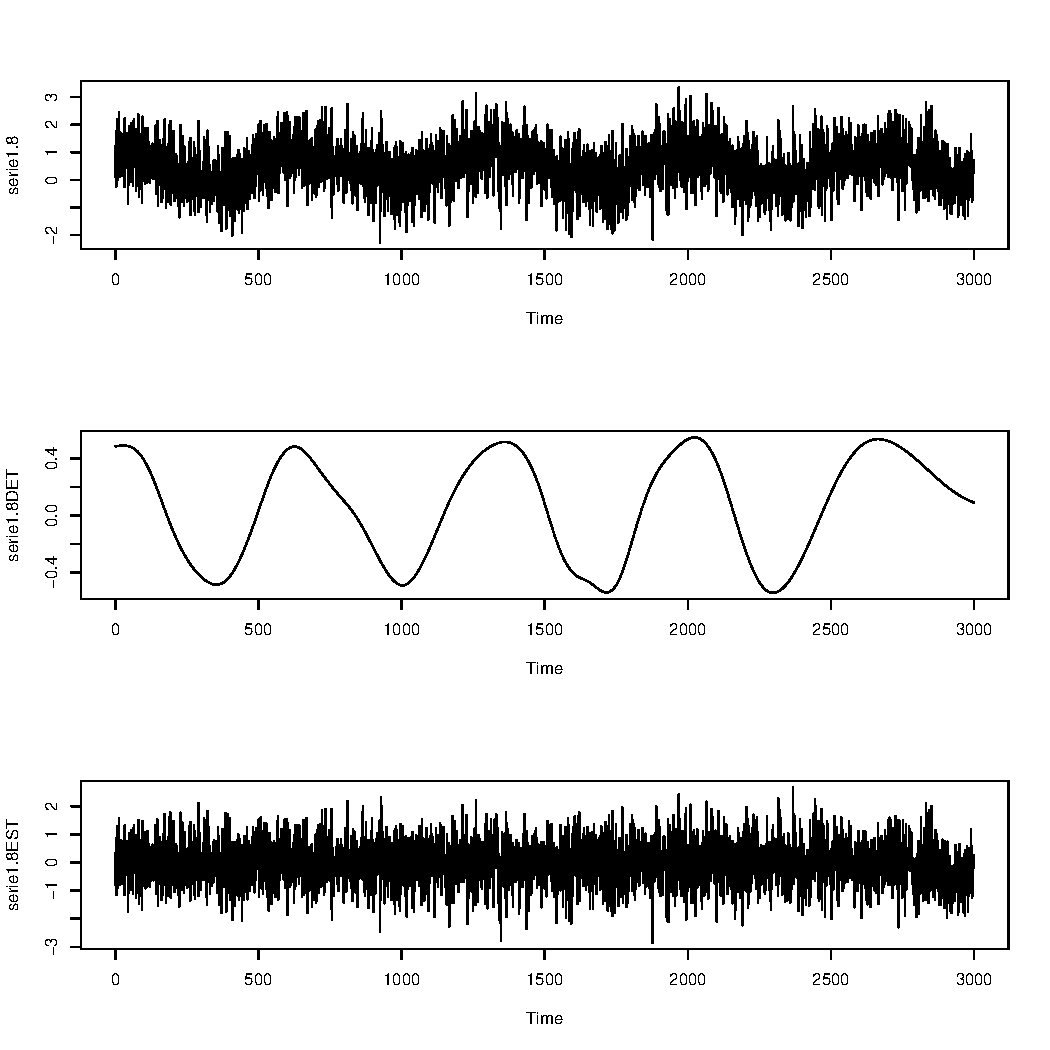
\includegraphics[scale=0.43]{serie1_8.pdf}
  \caption{Série 1.7 e Série 1.8}

\end{center}
\end{figure}

\graphicspath{{imagens/}}
\begin{figure}[H]
\begin{center}
  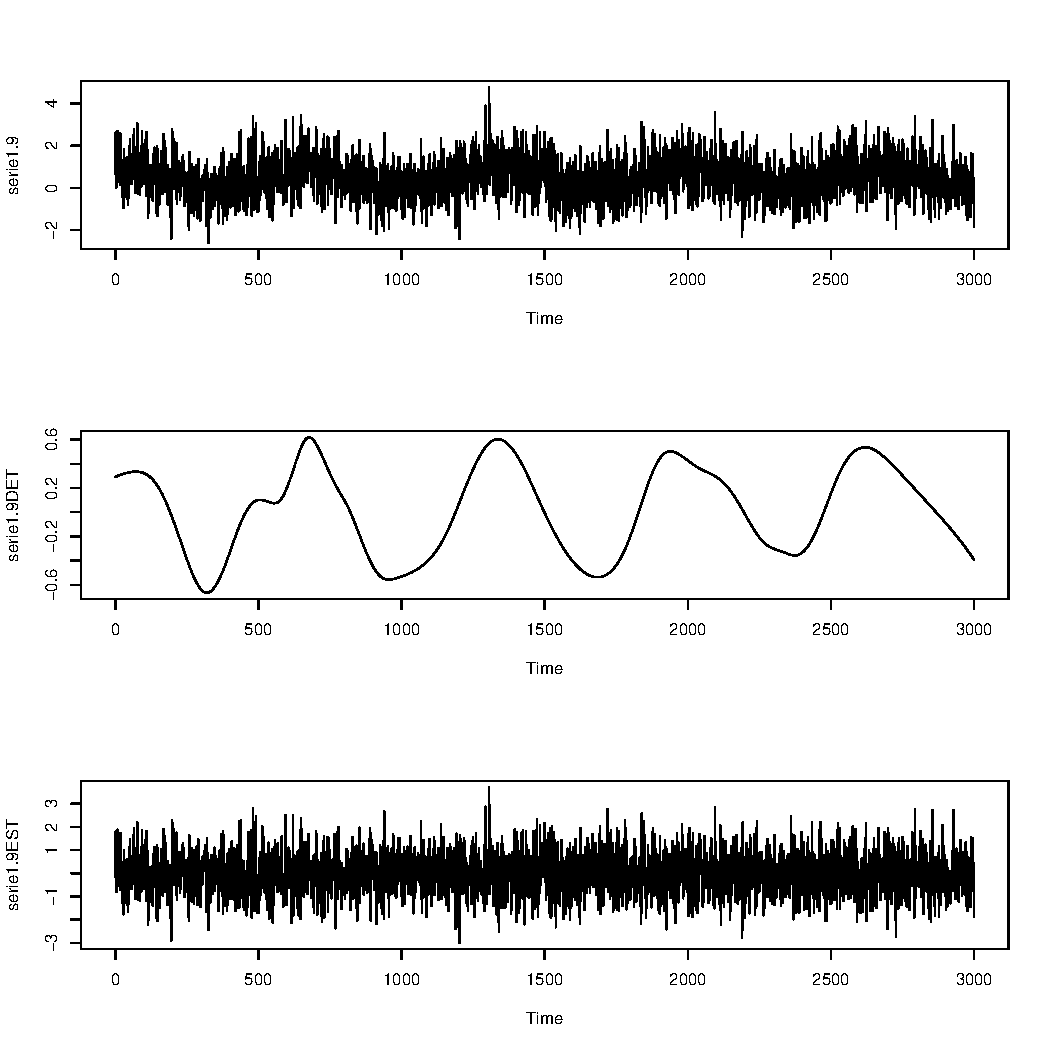
\includegraphics[scale=0.43]{serie1_9.pdf} \quad
  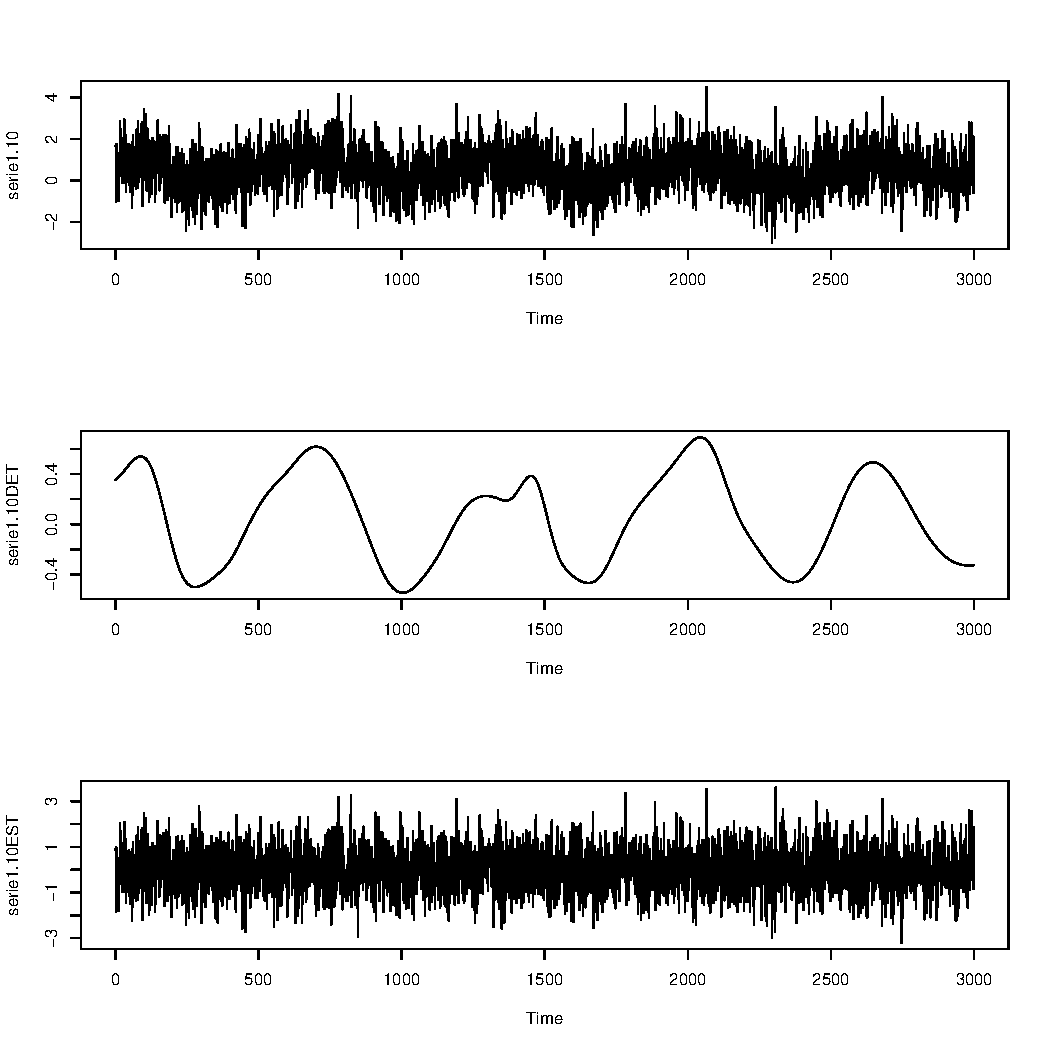
\includegraphics[scale=0.43]{serie1_10.pdf}
  \caption{Série 1.9 e Série 1.10}

\end{center}
\end{figure}

\section{Séries TIPO 2}
10 séries cossenoide com ruído ao longo da série e tendência.
\graphicspath{{imagens/}}
\begin{figure}[H]
\begin{center}
  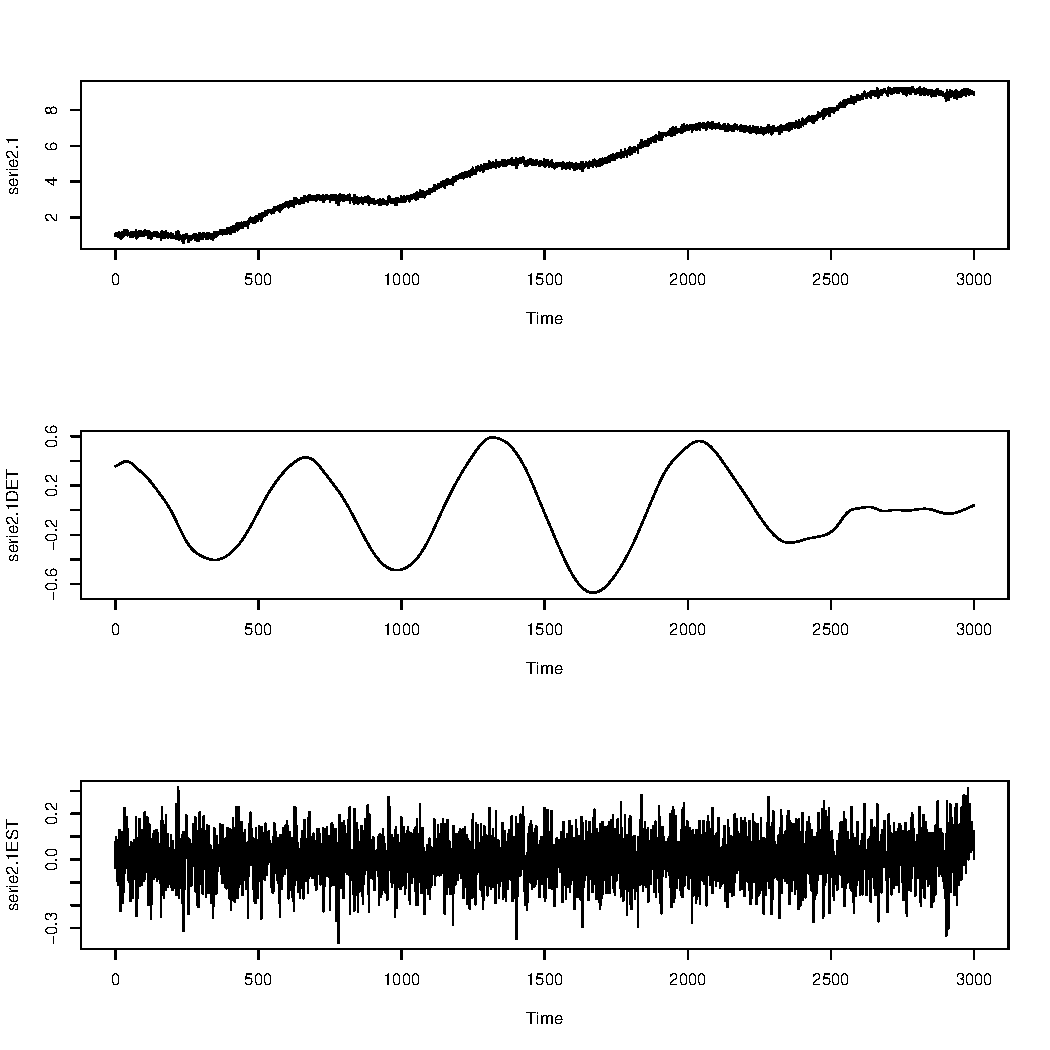
\includegraphics[scale=0.43]{serie2_1.pdf} \quad
  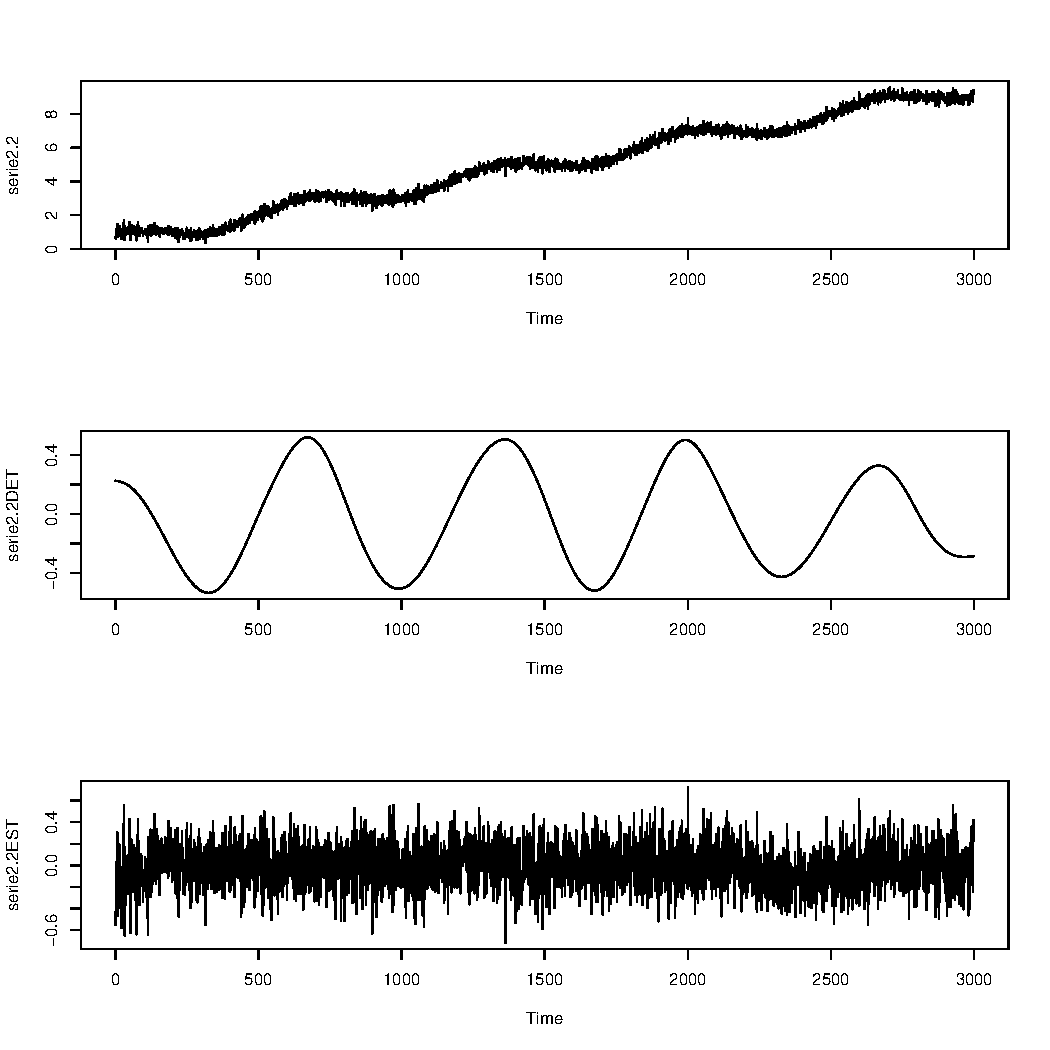
\includegraphics[scale=0.43]{serie2_2.pdf}
  \caption{Série 2.1 e Série 2.2}

\end{center}
\end{figure}

\graphicspath{{imagens/}}
\begin{figure}[H]
\begin{center}
  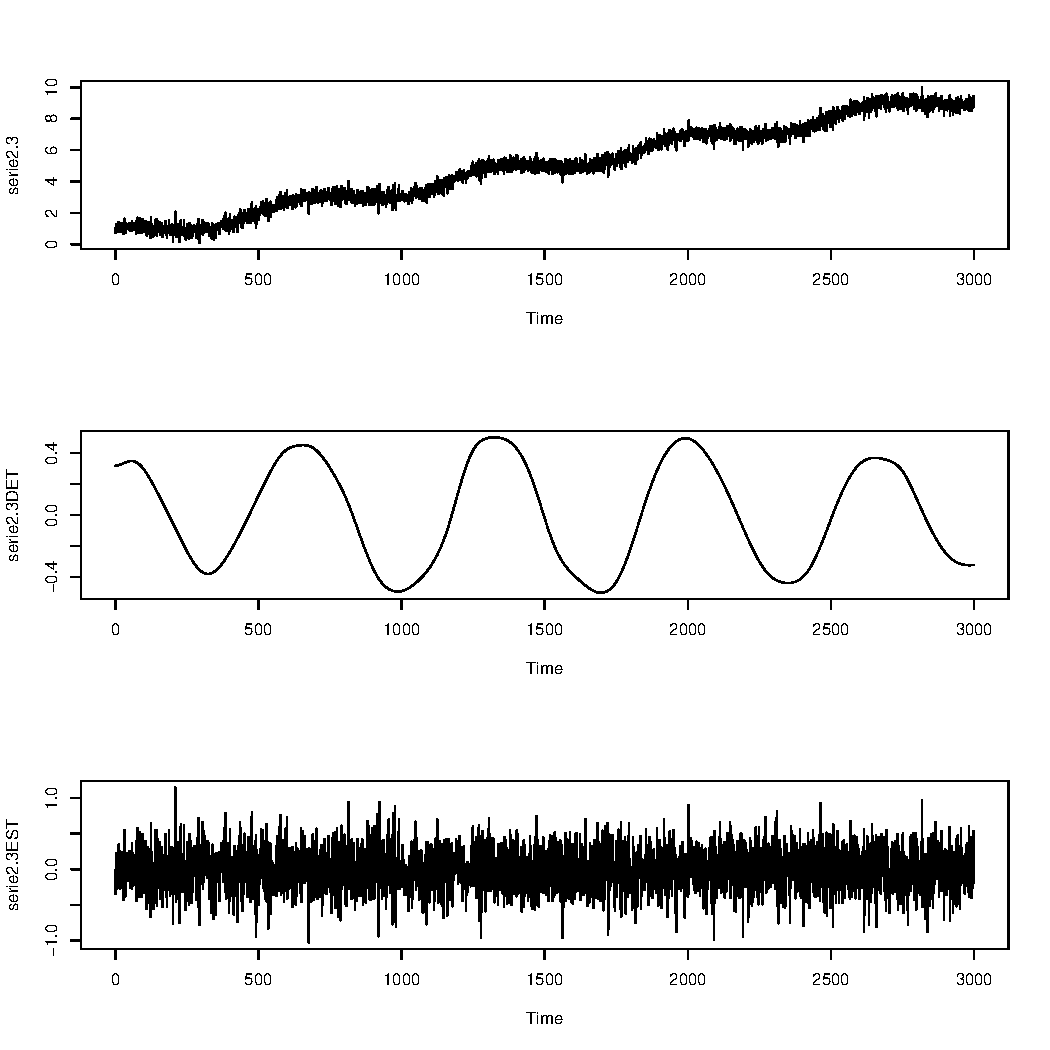
\includegraphics[scale=0.43]{serie2_3.pdf} \quad
  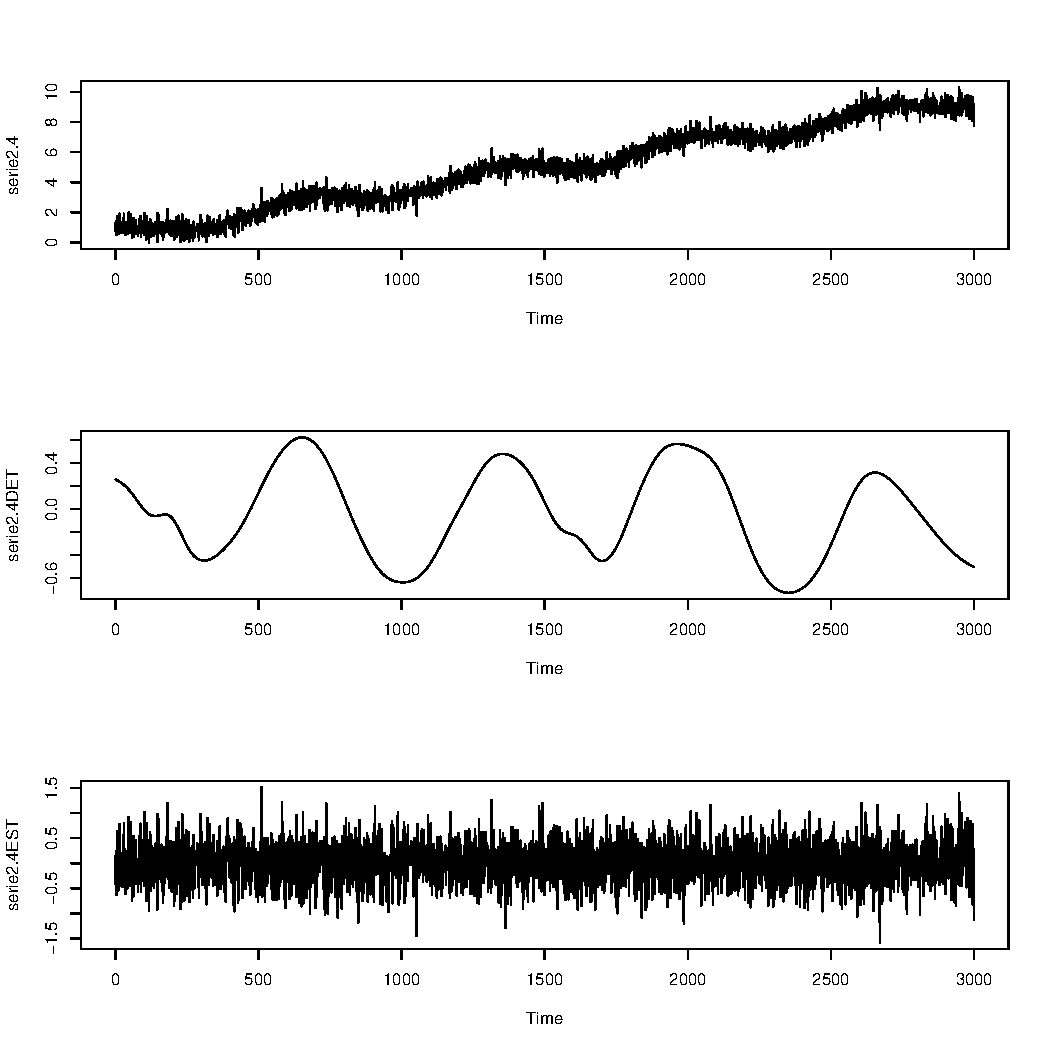
\includegraphics[scale=0.43]{serie2_4.pdf}
  \caption{Série 2.3 e Série 2.4}

\end{center}
\end{figure}

\graphicspath{{imagens/}}
\begin{figure}[H]
\begin{center}
  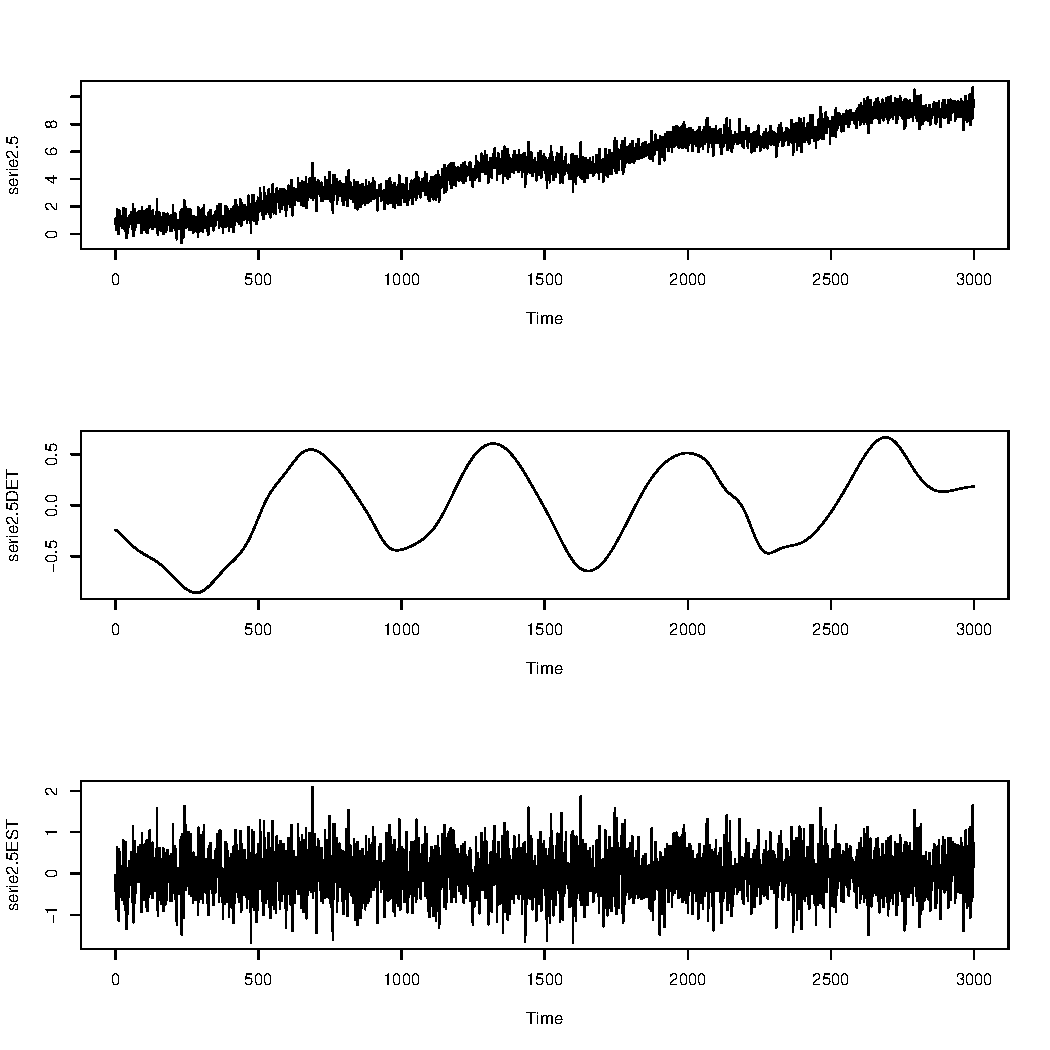
\includegraphics[scale=0.43]{serie2_5.pdf} \quad
  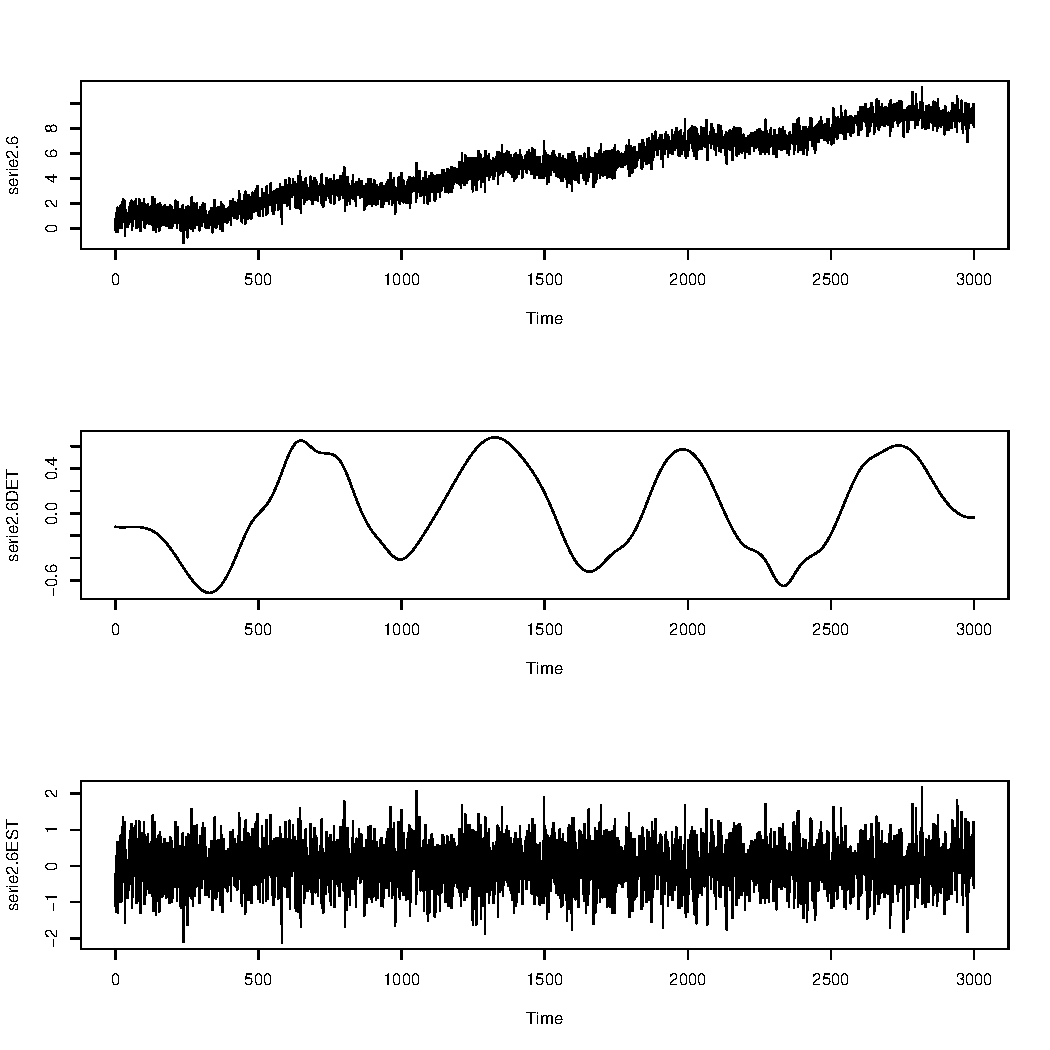
\includegraphics[scale=0.43]{serie2_6.pdf}
  \caption{Série 2.5 e Série 2.6}

\end{center}
\end{figure}

\graphicspath{{imagens/}}
\begin{figure}[H]
\begin{center}
  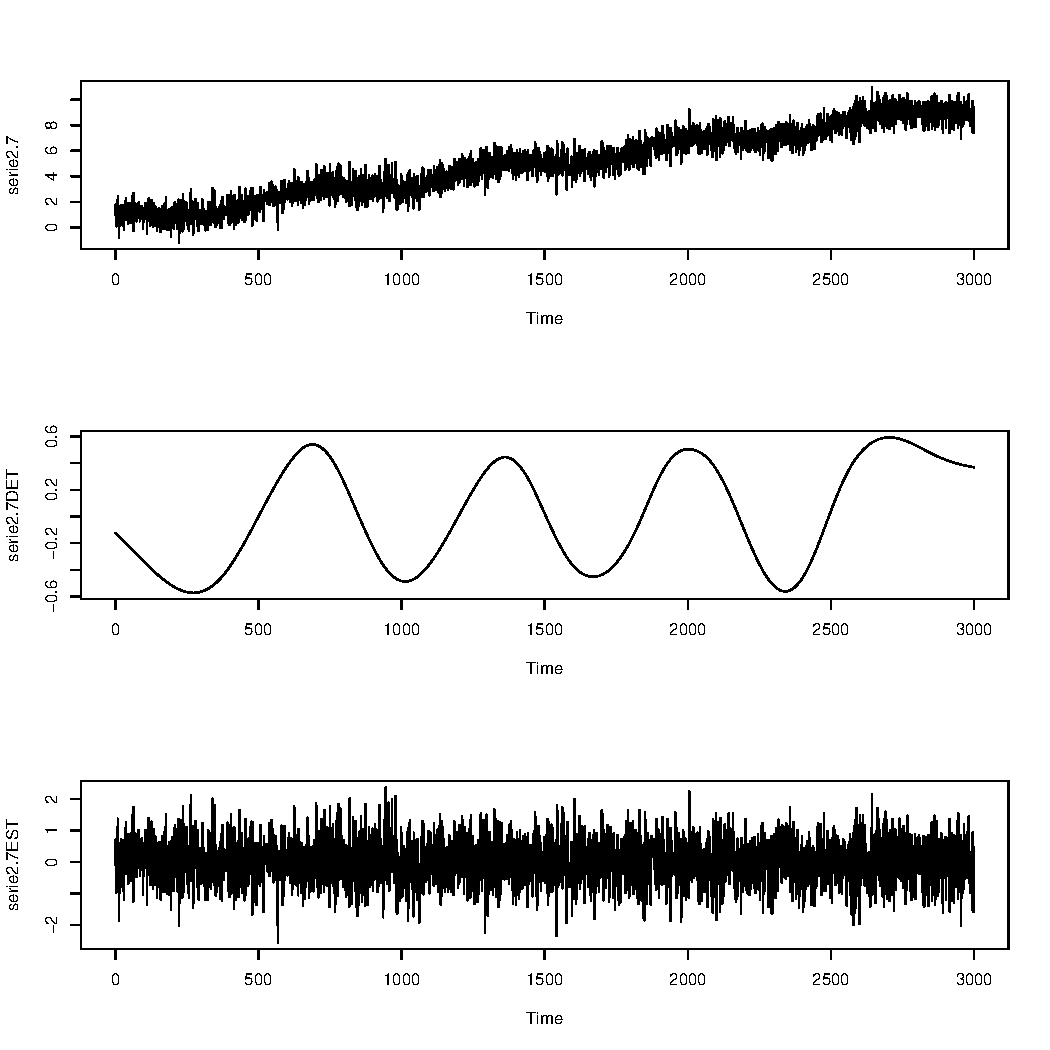
\includegraphics[scale=0.43]{serie2_7.pdf} \quad
  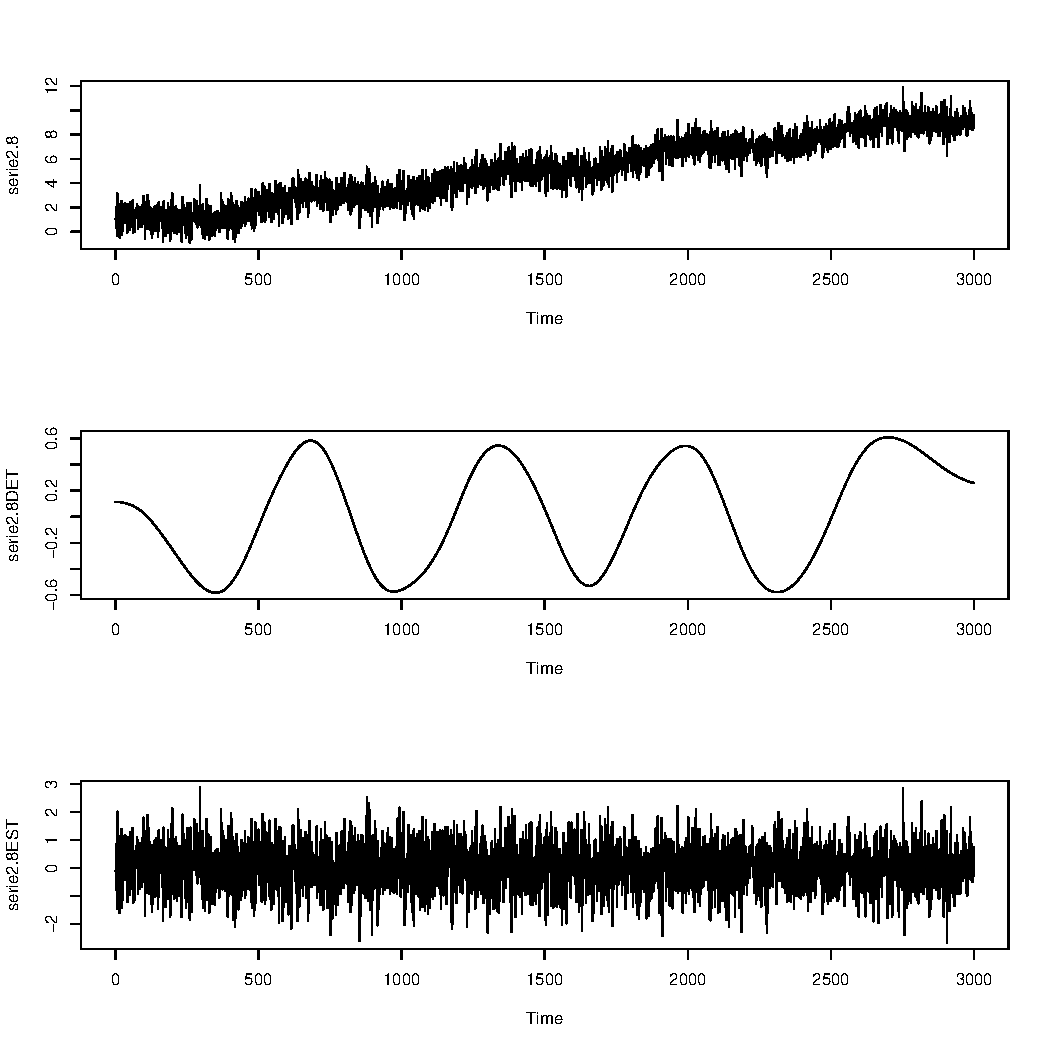
\includegraphics[scale=0.43]{serie2_8.pdf}
  \caption{Série 2.7 e Série 2.8}

\end{center}
\end{figure}

\graphicspath{{imagens/}}
\begin{figure}[H]
\begin{center}
  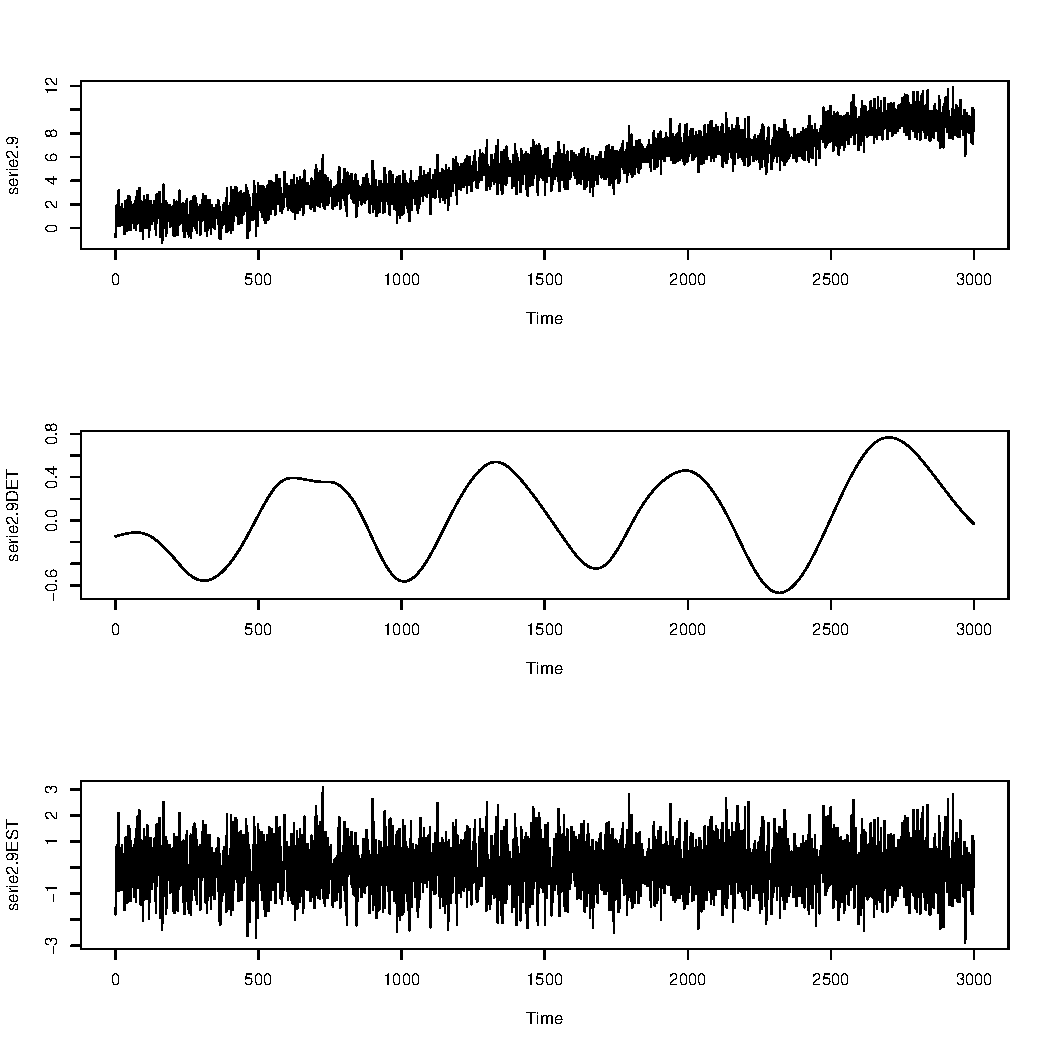
\includegraphics[scale=0.43]{serie2_9.pdf} \quad
  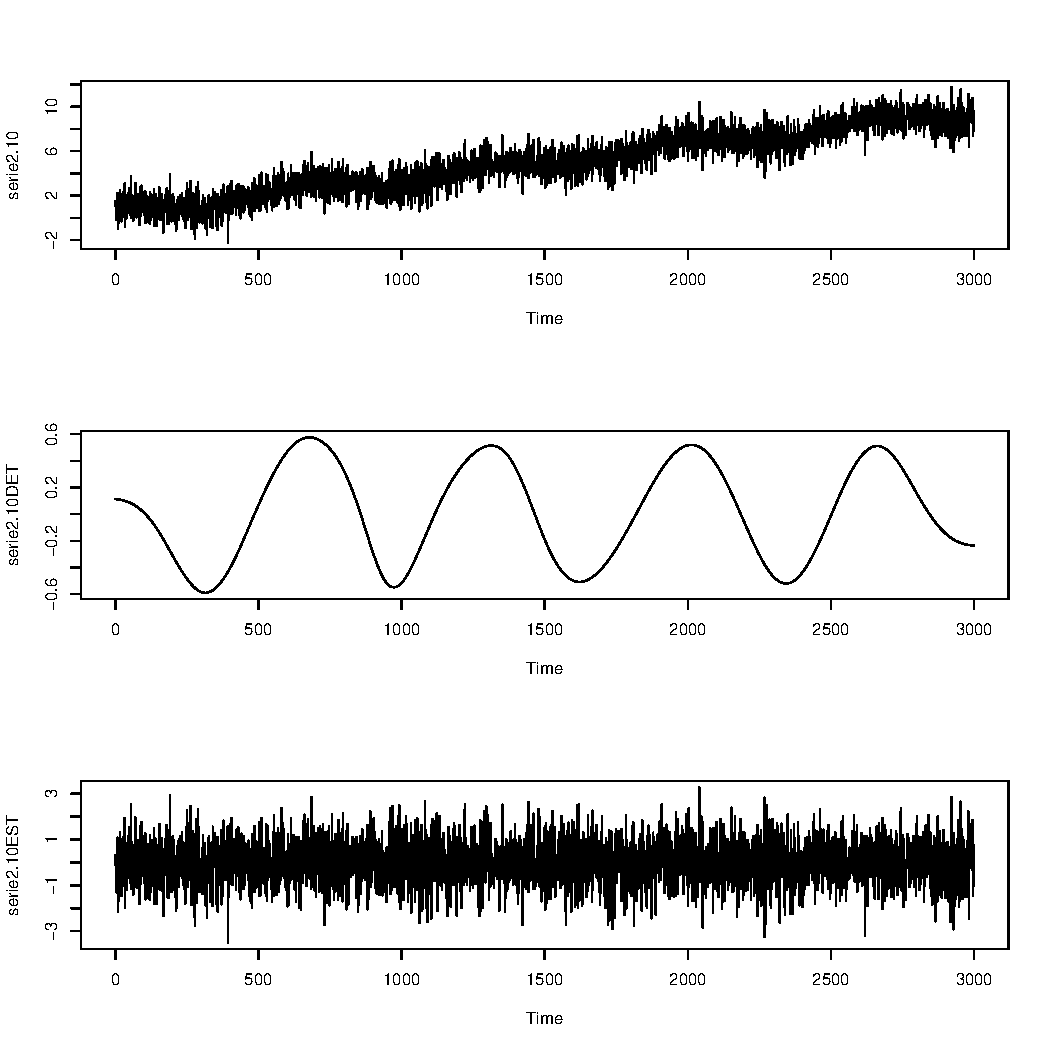
\includegraphics[scale=0.43]{serie2_10.pdf}
  \caption{Série 2.9 e Série 2.10}

\end{center}
\end{figure}

\section{Séries TIPO 3}
10 séries senoide com ruído ao longo da série.
\graphicspath{{imagens/}}
\begin{figure}[H]
\begin{center}
  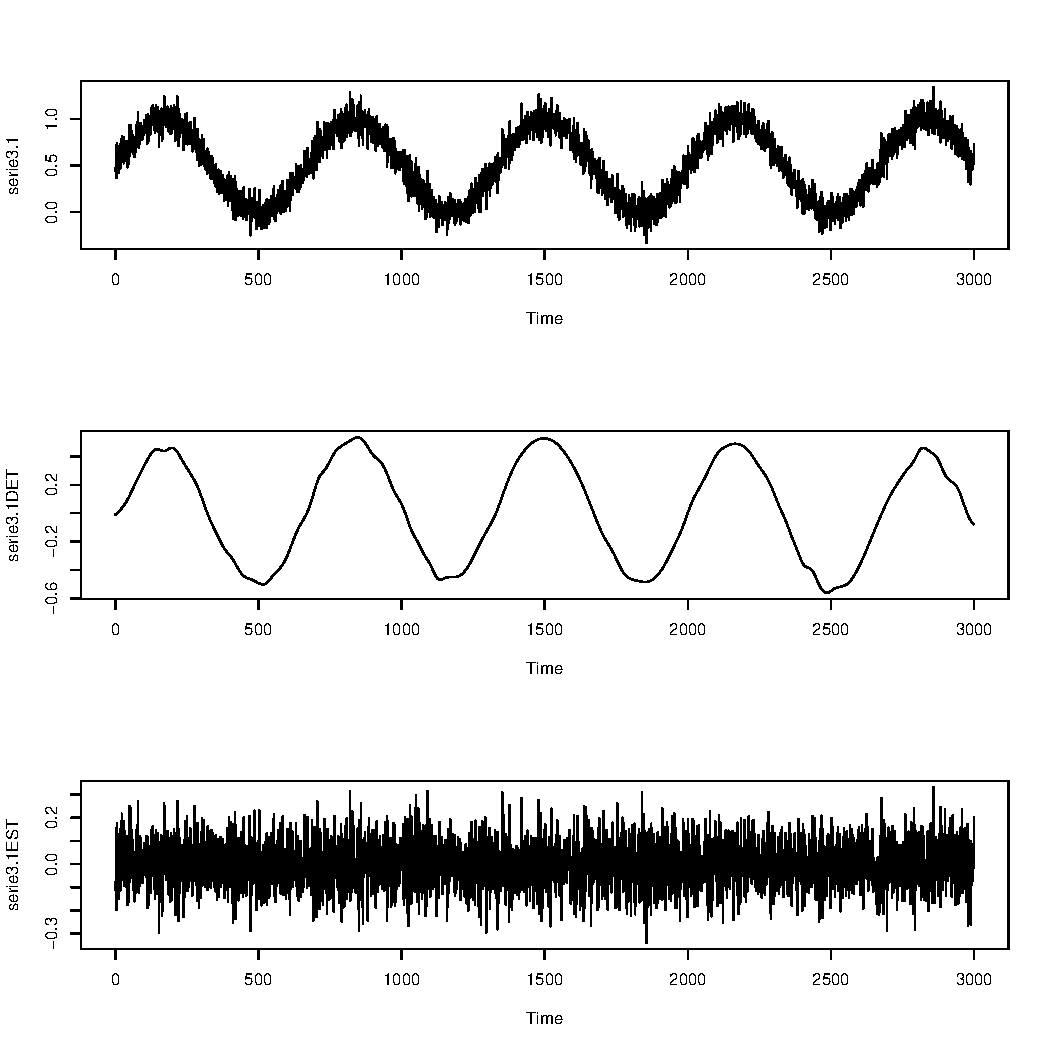
\includegraphics[scale=0.43]{serie3_1.pdf} \quad
  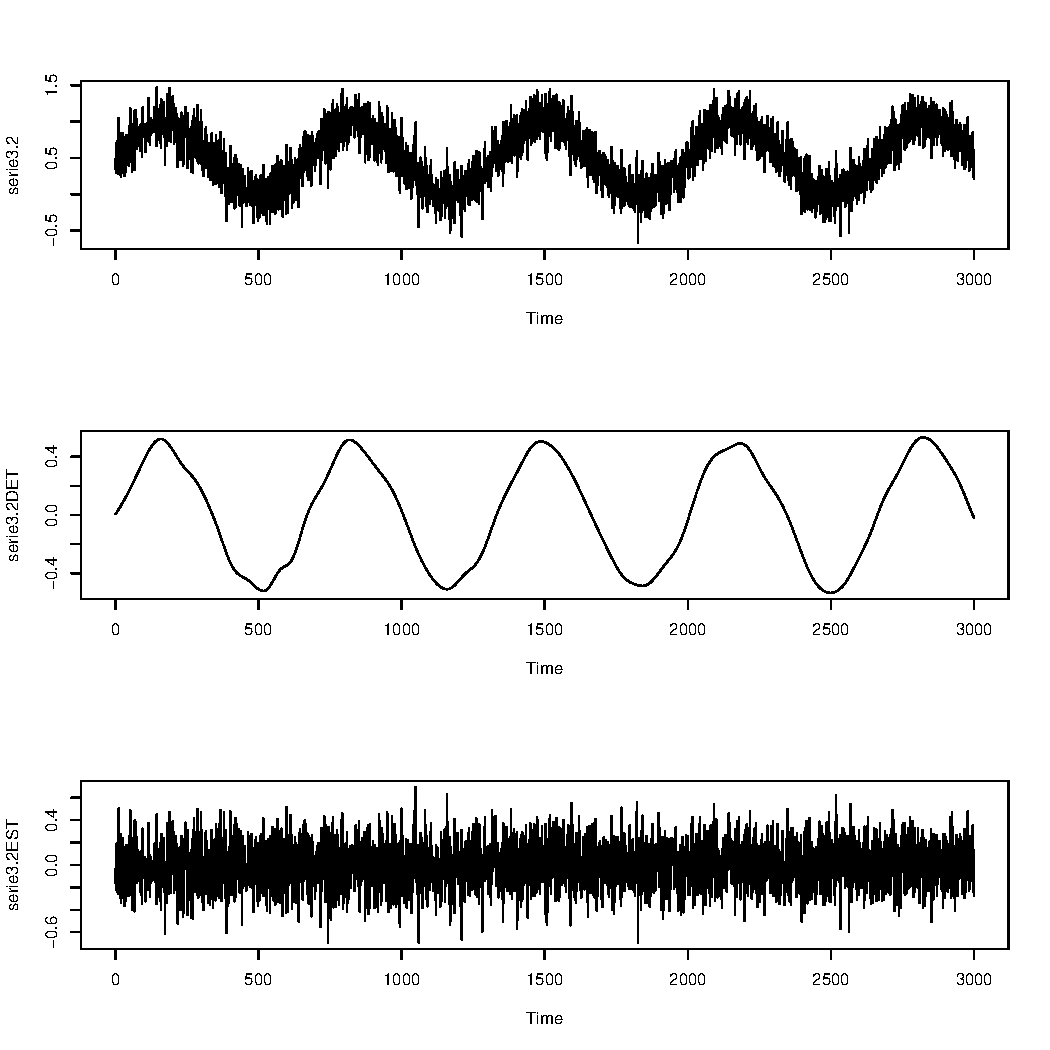
\includegraphics[scale=0.43]{serie3_2.pdf}
  \caption{Série 3.1 e Série 3.2}

\end{center}
\end{figure}

\graphicspath{{imagens/}}
\begin{figure}[H]
\begin{center}
  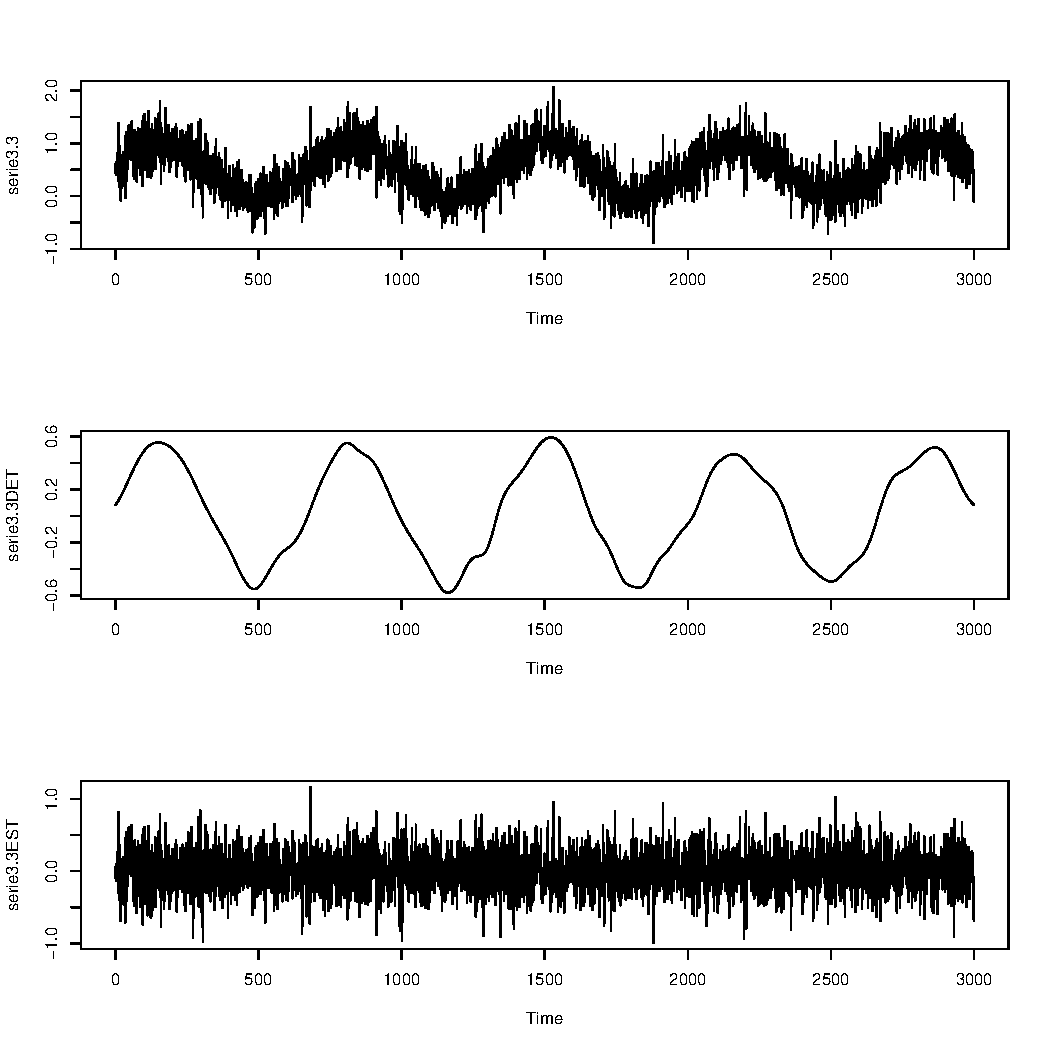
\includegraphics[scale=0.43]{serie3_3.pdf} \quad
  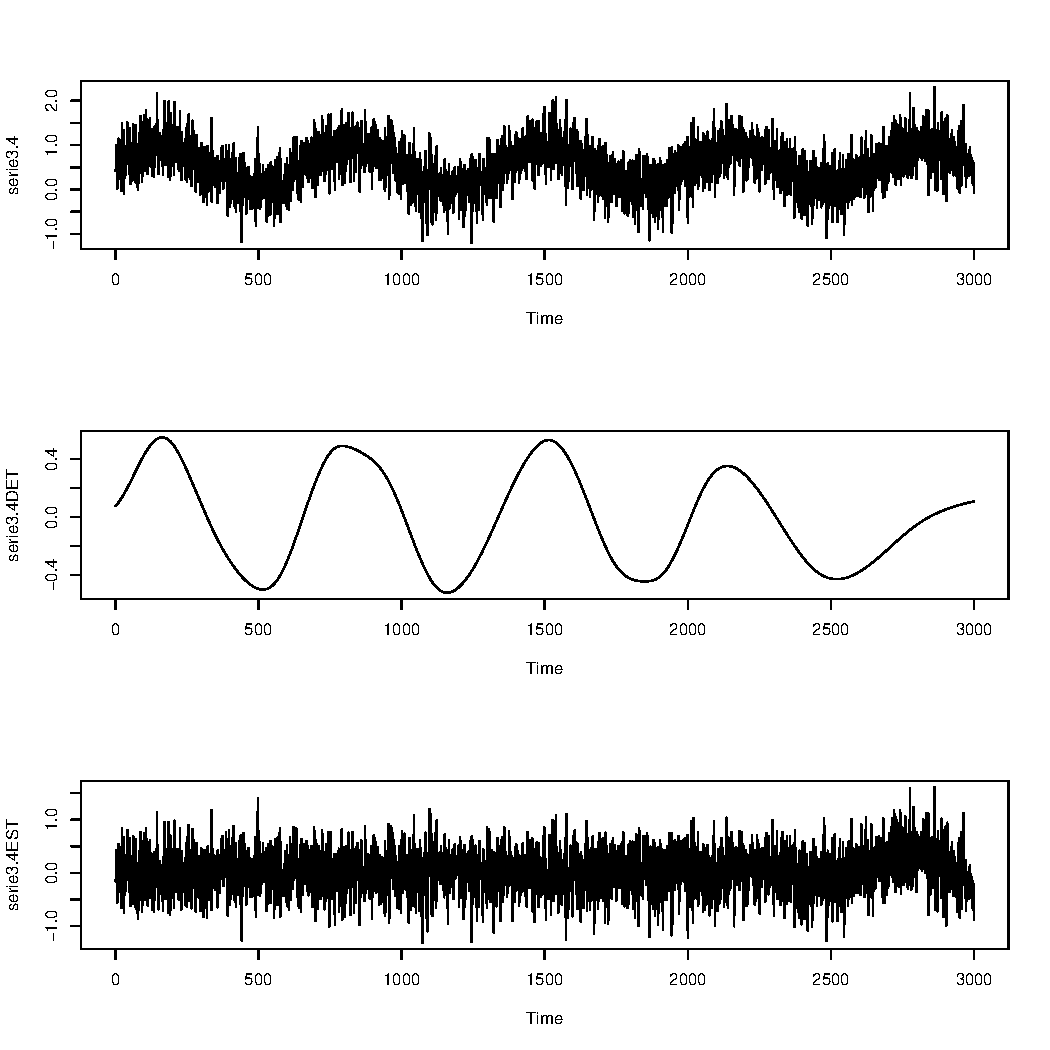
\includegraphics[scale=0.43]{serie3_4.pdf}
  \caption{Série 3.3 e Série 3.4}

\end{center}
\end{figure}

\graphicspath{{imagens/}}
\begin{figure}[H]
\begin{center}
  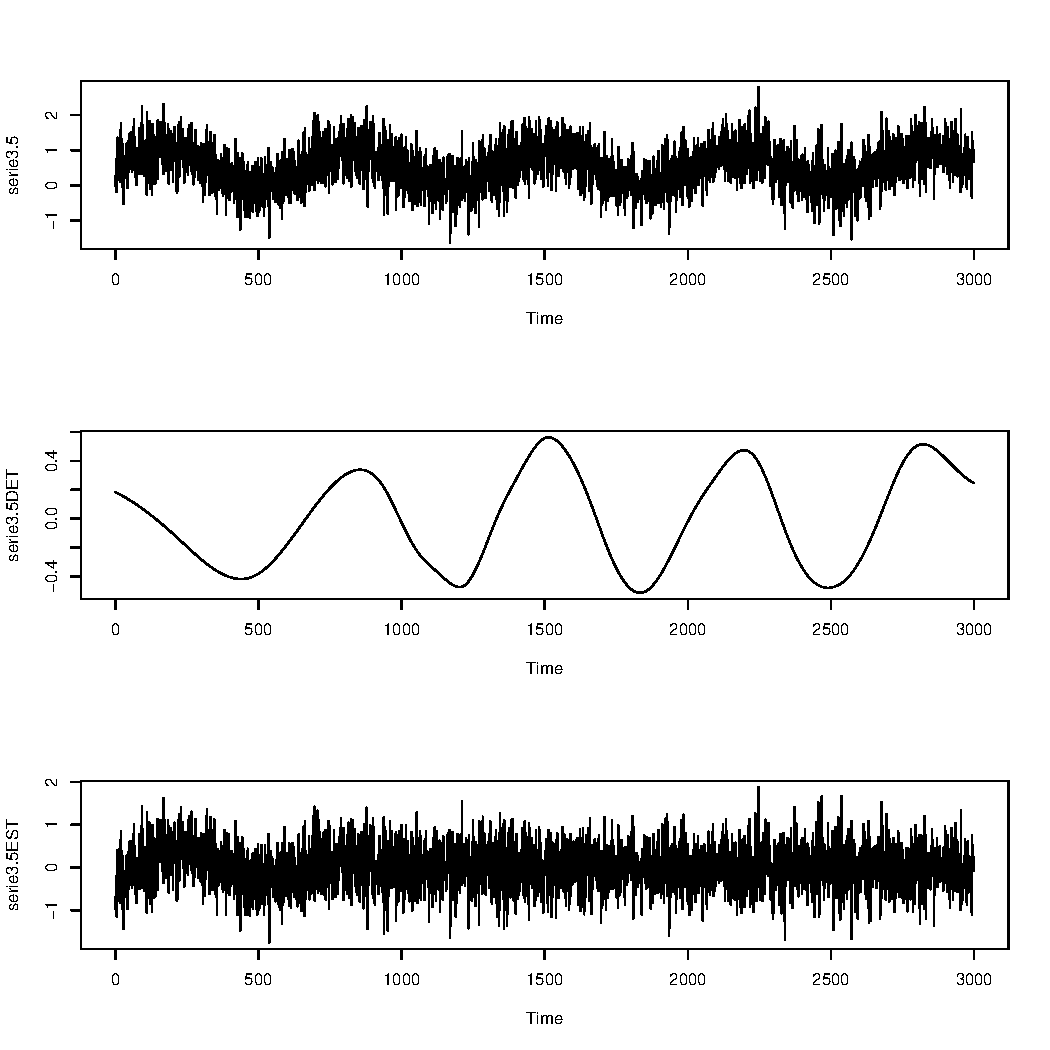
\includegraphics[scale=0.43]{serie3_5.pdf} \quad
  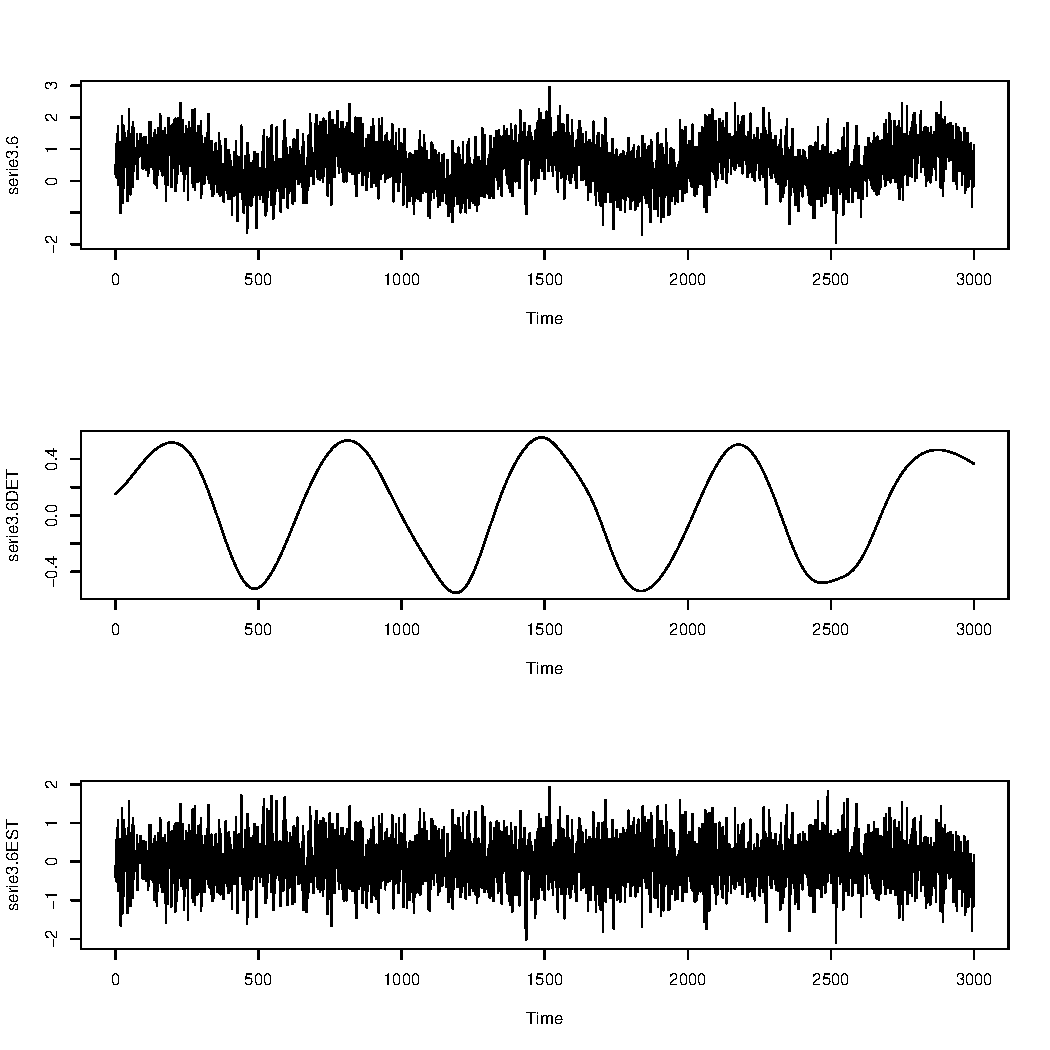
\includegraphics[scale=0.43]{serie3_6.pdf}
  \caption{Série 3.5 e Série 3.6}

\end{center}
\end{figure}

\graphicspath{{imagens/}}
\begin{figure}[H]
\begin{center}
  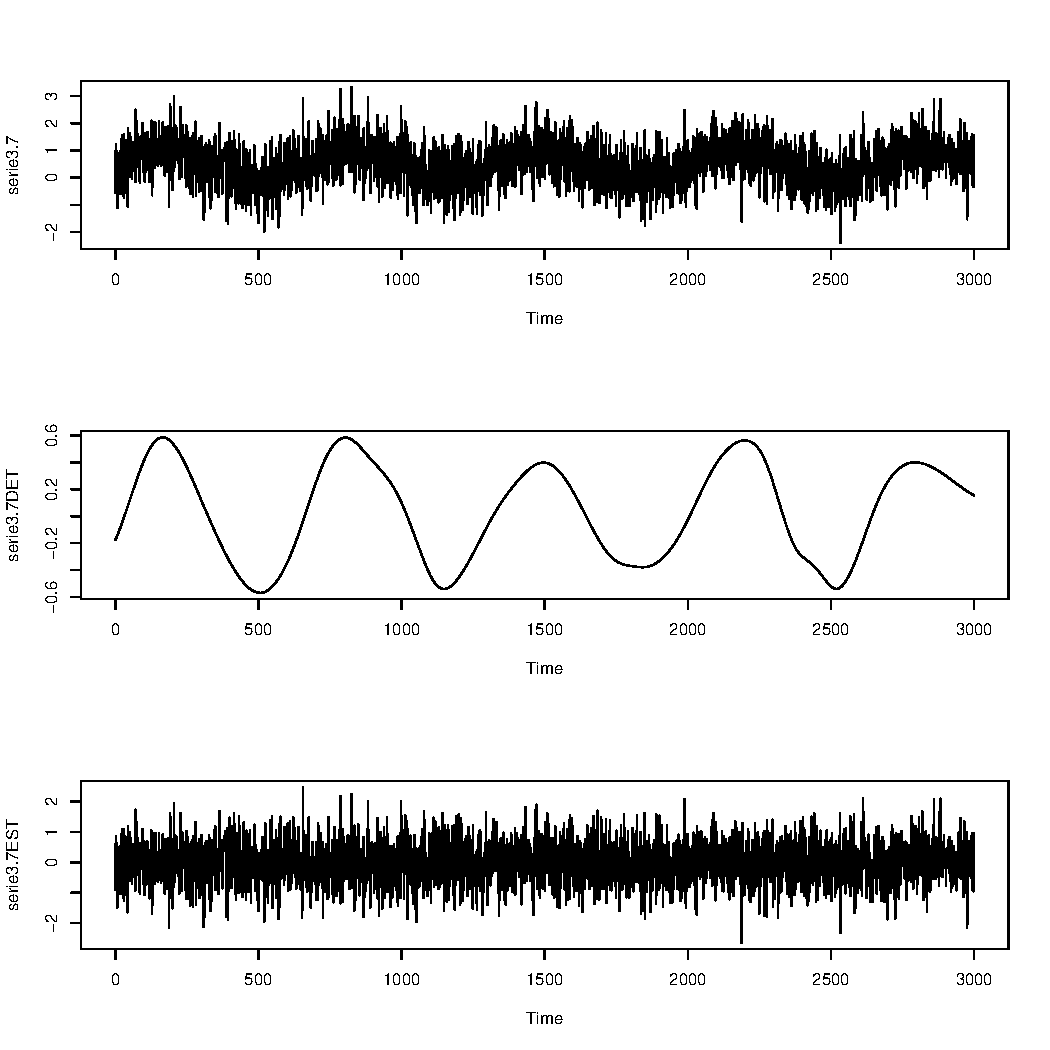
\includegraphics[scale=0.43]{serie3_7.pdf} \quad
  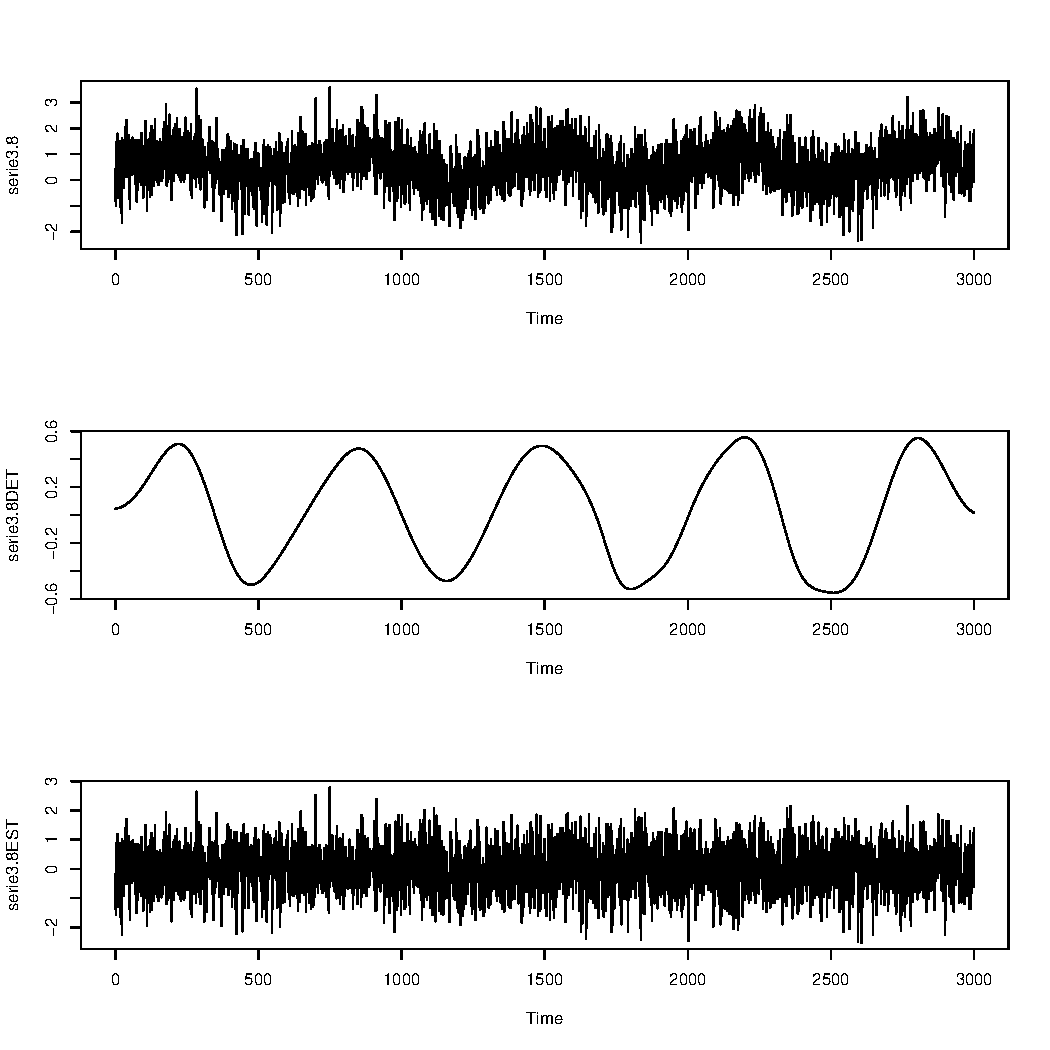
\includegraphics[scale=0.43]{serie3_8.pdf}
  \caption{Série 3.7 e Série 3.8}

\end{center}
\end{figure}

\graphicspath{{imagens/}}
\begin{figure}[H]
\begin{center}
  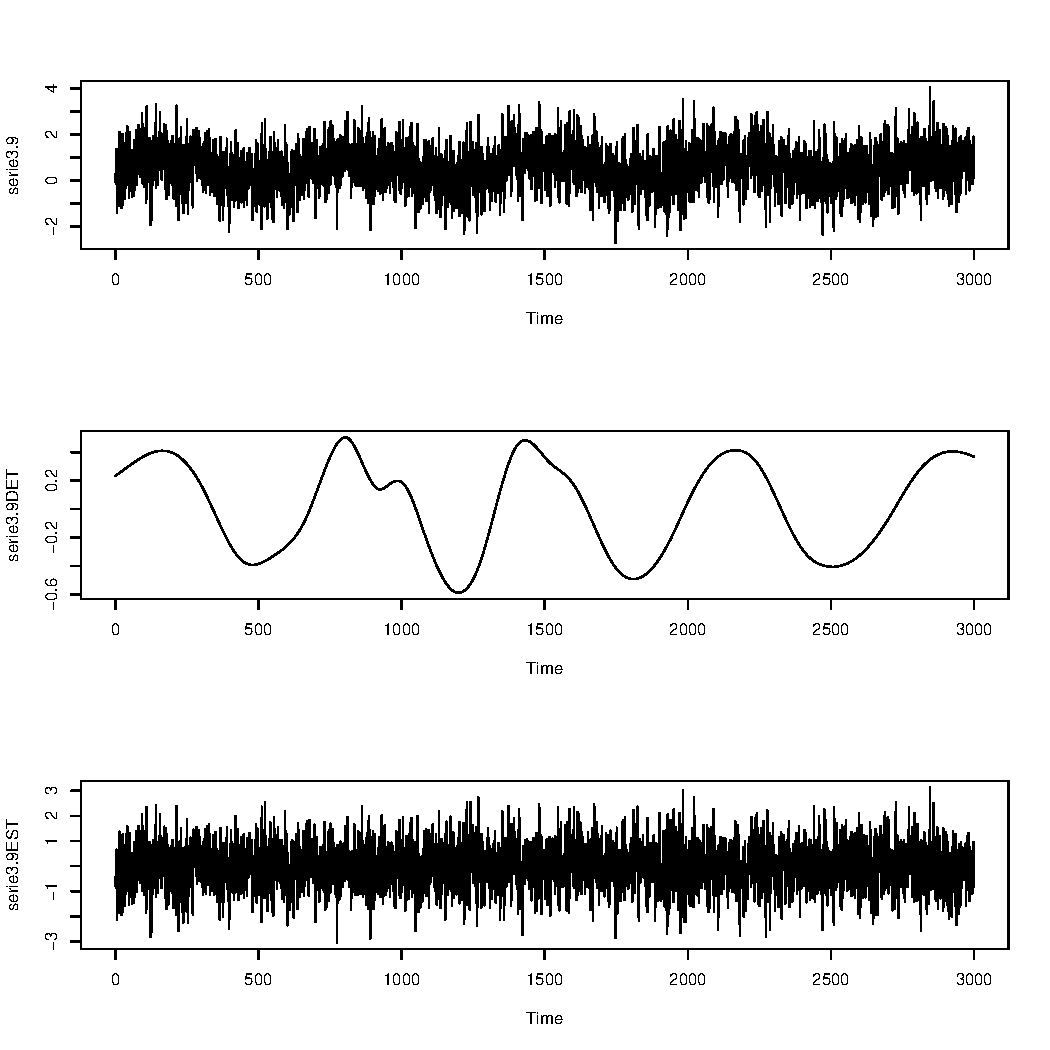
\includegraphics[scale=0.43]{serie3_9.pdf} \quad
  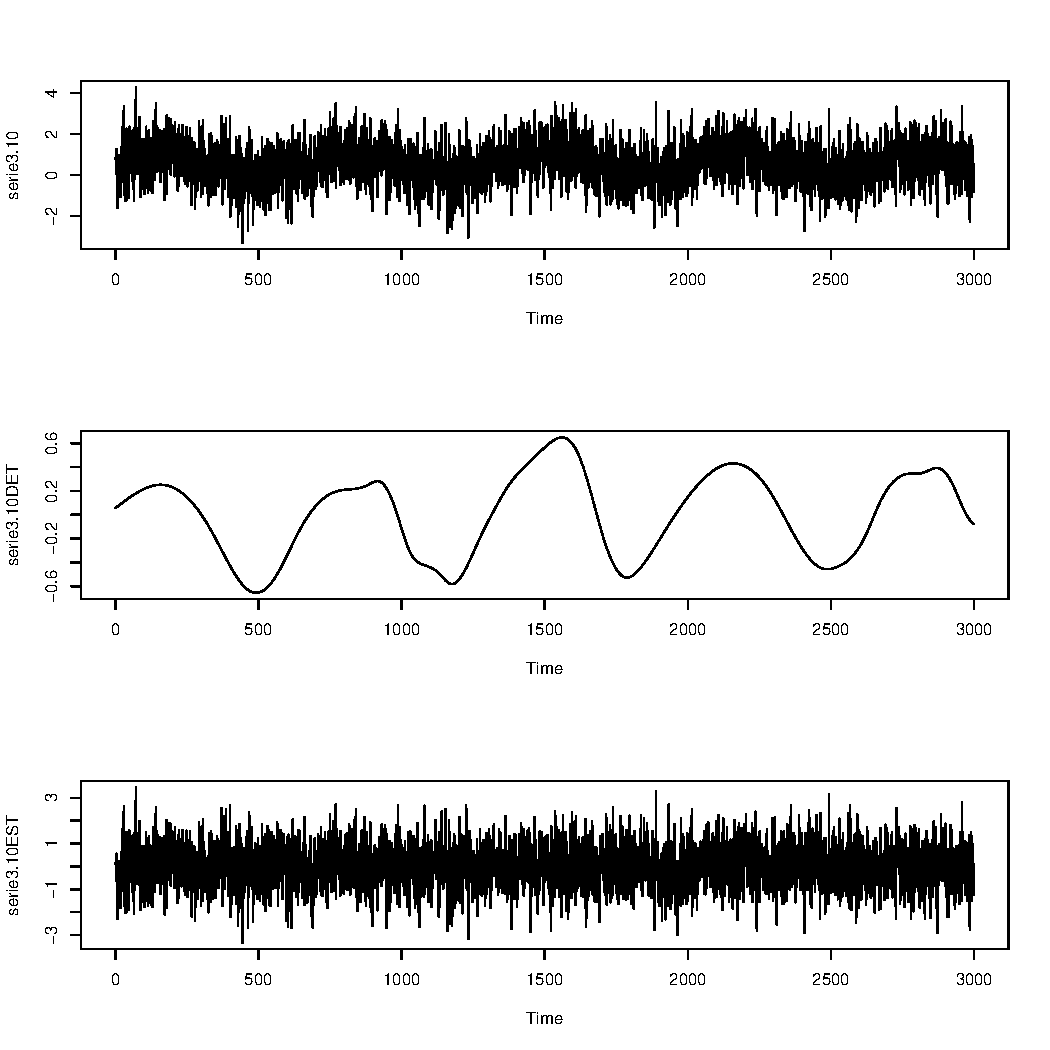
\includegraphics[scale=0.43]{serie3_10.pdf}
  \caption{Série 3.9 e Série 3.10}

\end{center}
\end{figure}

\section{Séries TIPO 4}
10 séries senoide com ruído ao longo da série e tendência.
\graphicspath{{imagens/}}
\begin{figure}[H]
\begin{center}
  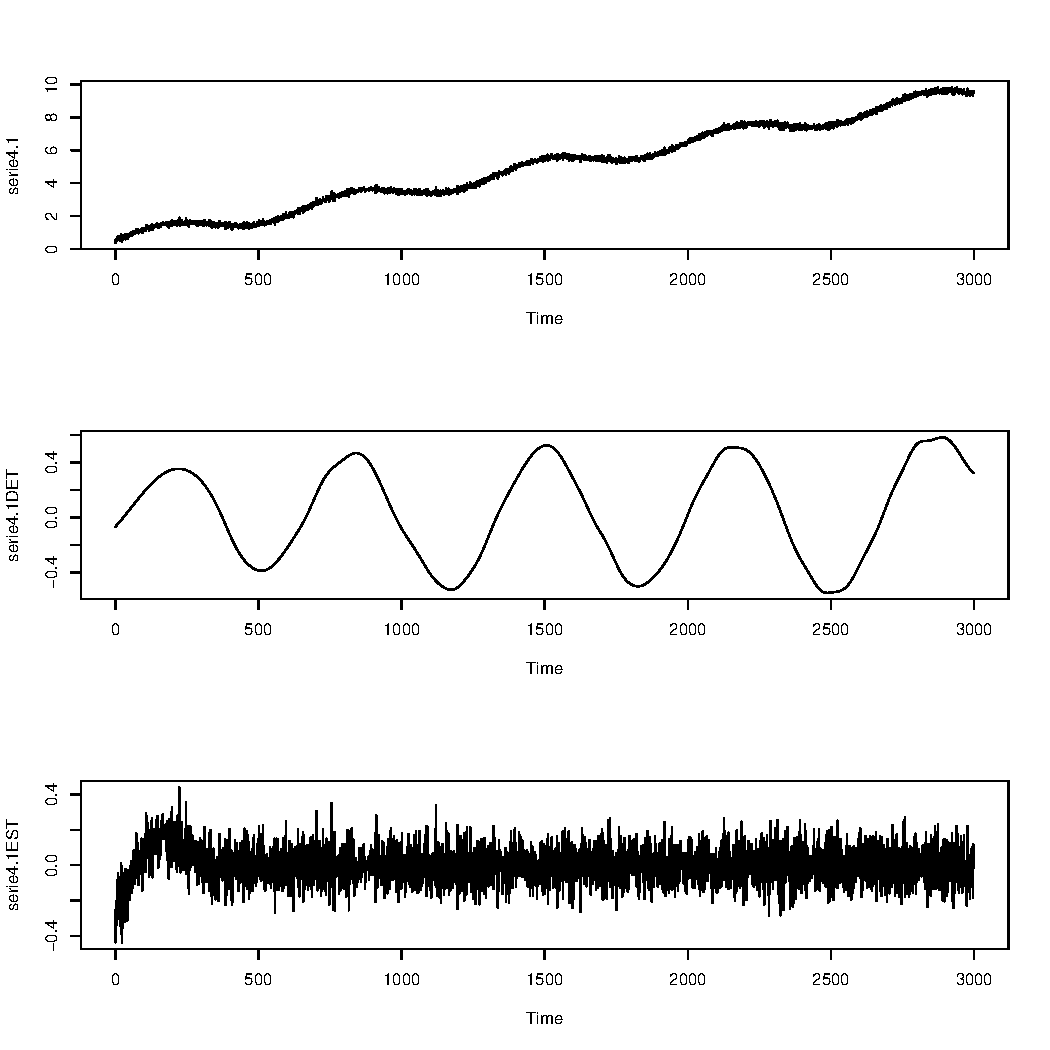
\includegraphics[scale=0.43]{serie4_1.pdf} \quad
  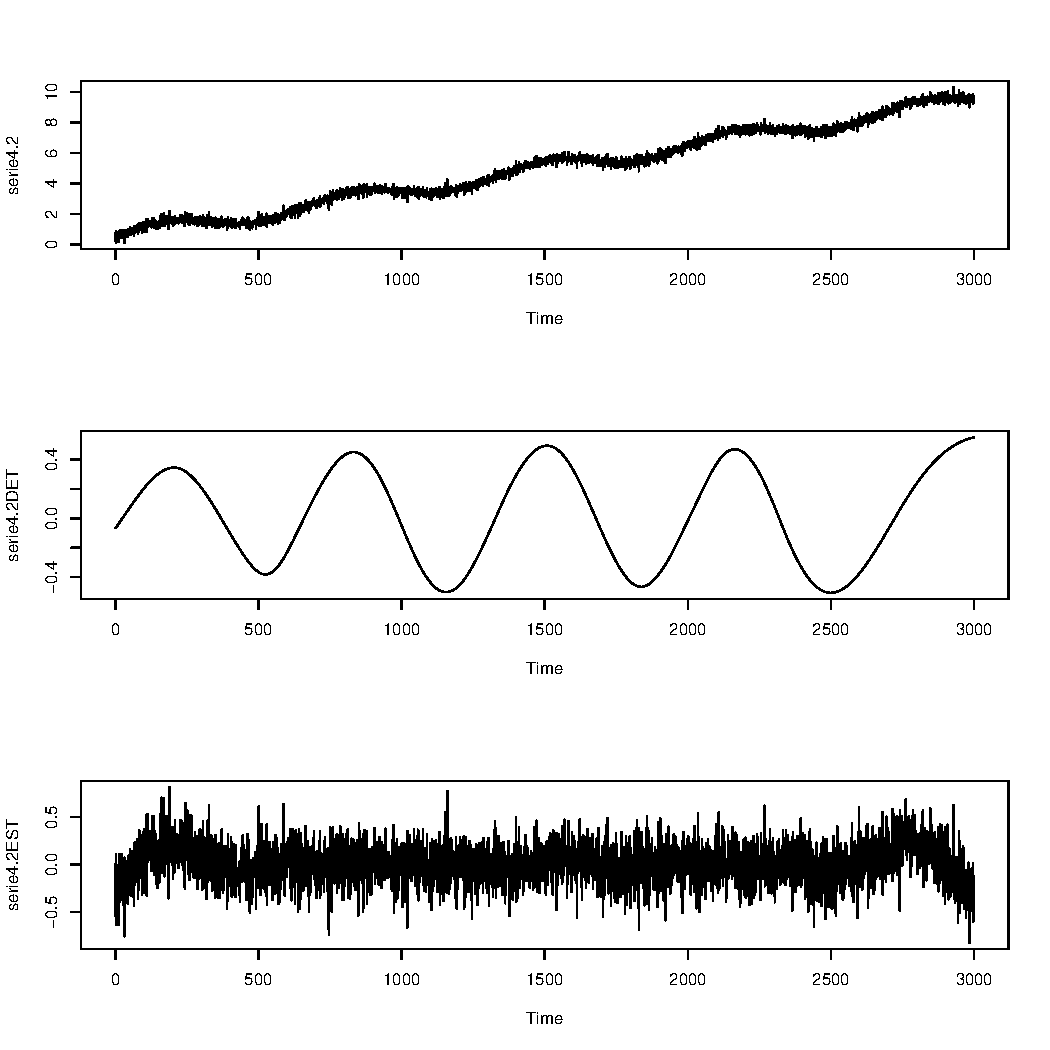
\includegraphics[scale=0.43]{serie4_2.pdf}
  \caption{Série 4.1 e Série 4.2}
\end{center}
\end{figure}

\graphicspath{{imagens/}}
\begin{figure}[H]
\begin{center}
  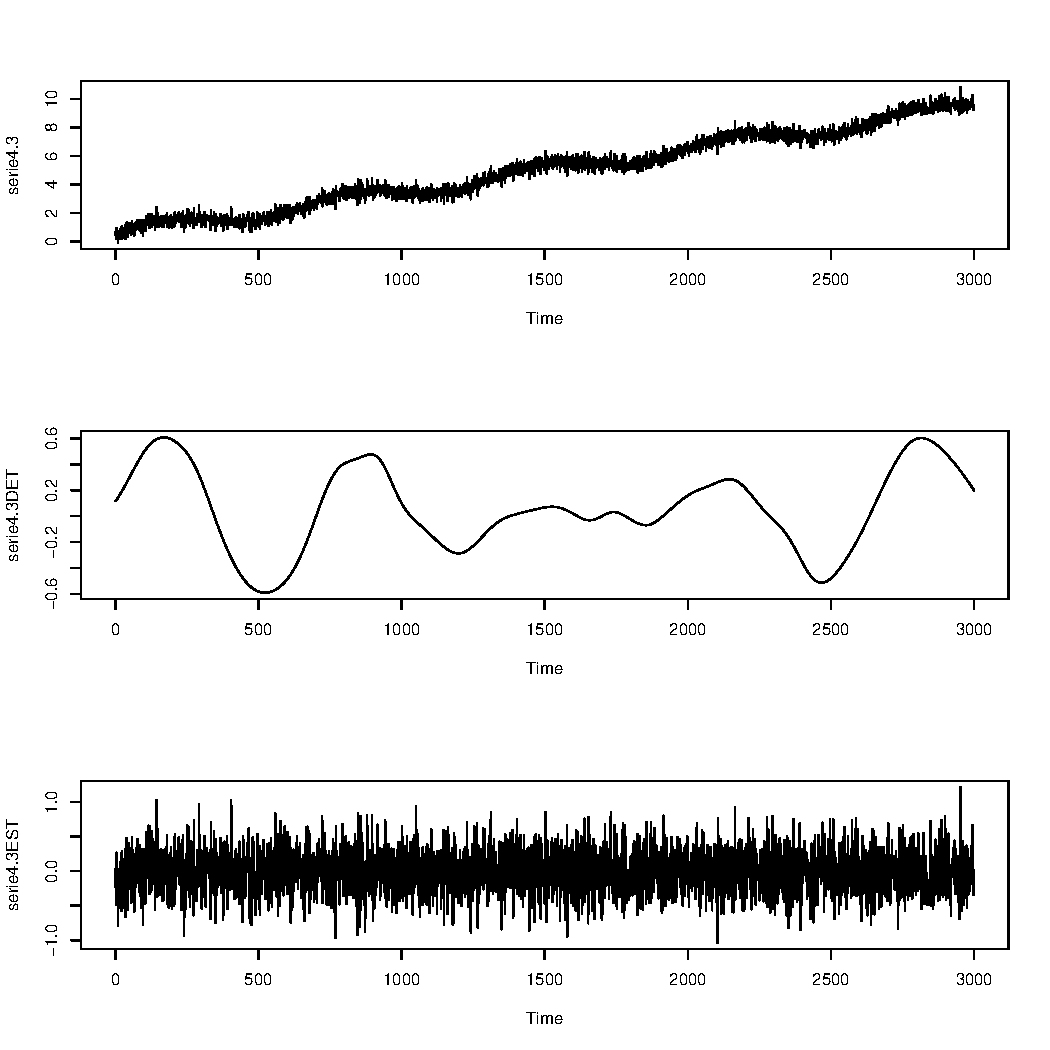
\includegraphics[scale=0.43]{serie4_3.pdf} \quad
 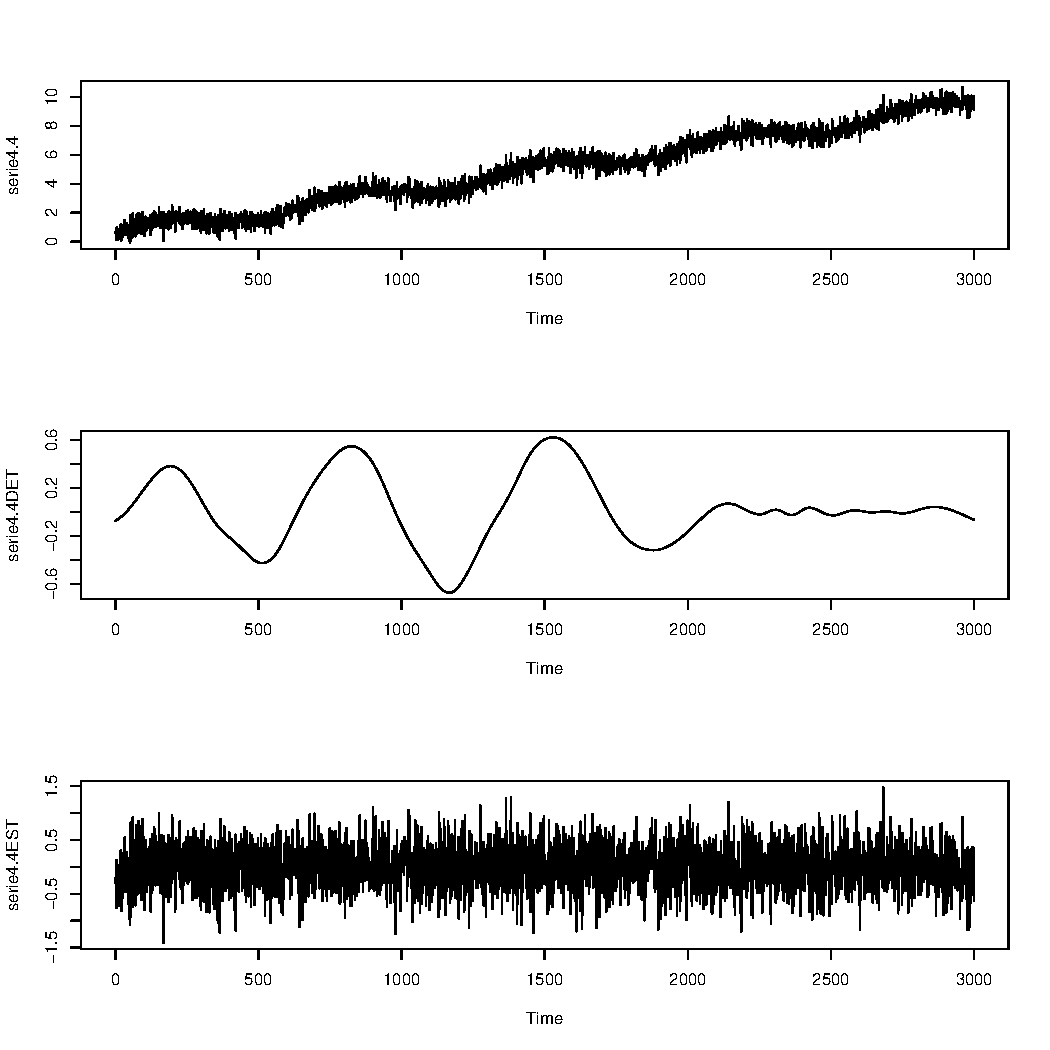
\includegraphics[scale=0.43]{serie4_4.pdf}
 \caption{Série 4.3 e Série 4.4}

\end{center}
\end{figure}

\graphicspath{{imagens/}}
\begin{figure}[H]
\begin{center}
  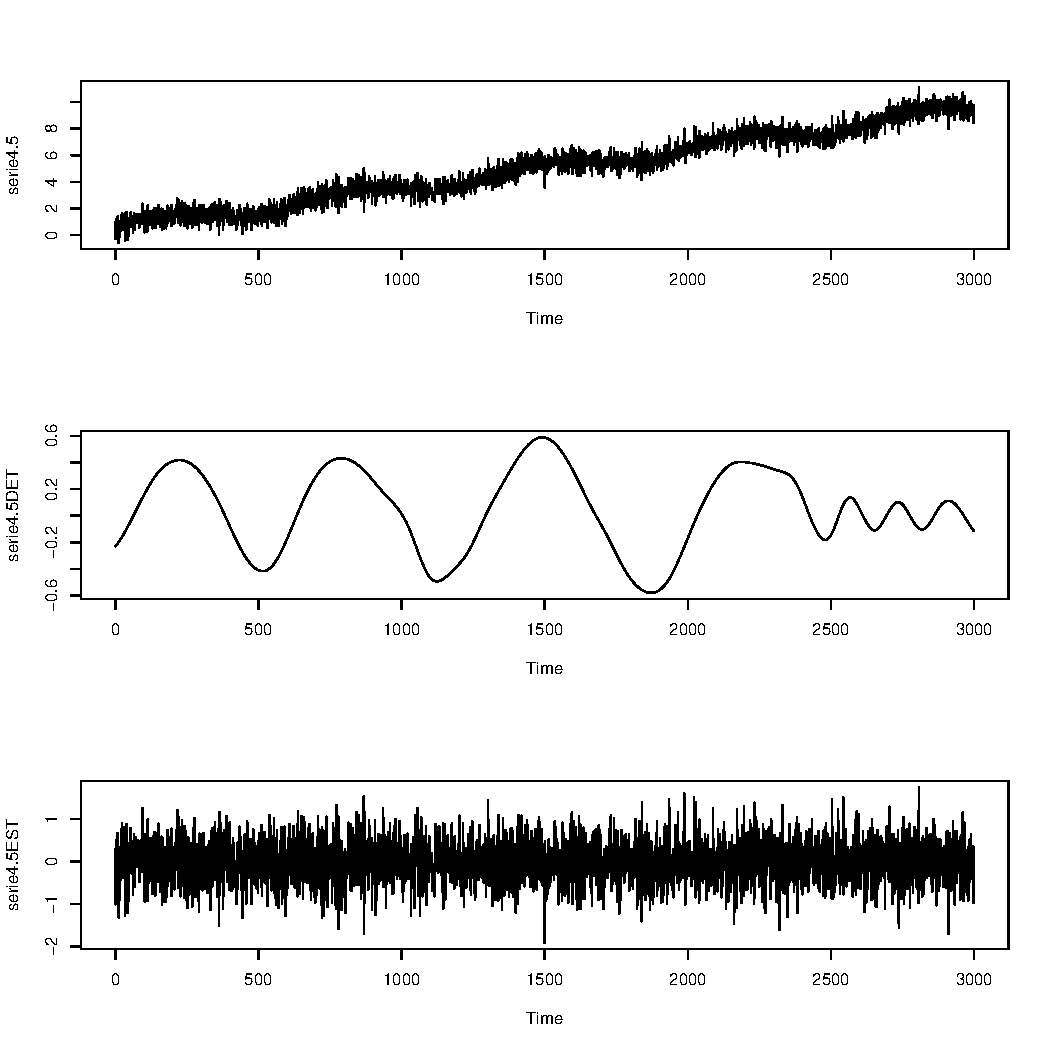
\includegraphics[scale=0.43]{serie4_5.pdf} \quad
  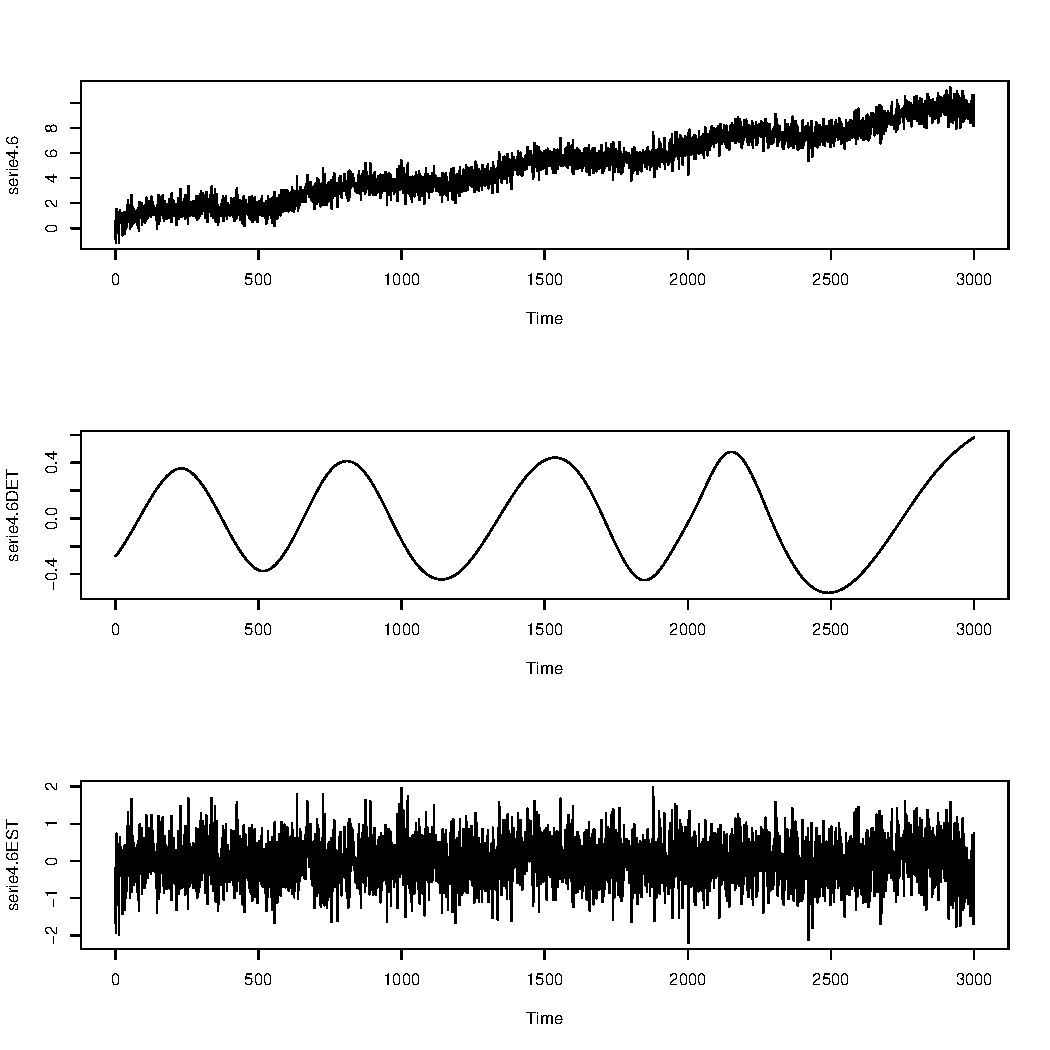
\includegraphics[scale=0.43]{serie4_6.pdf}
 \caption{Série 4.5 e Série 4.6}

\end{center}
\end{figure}

\graphicspath{{imagens/}}
\begin{figure}[H]
\begin{center}
  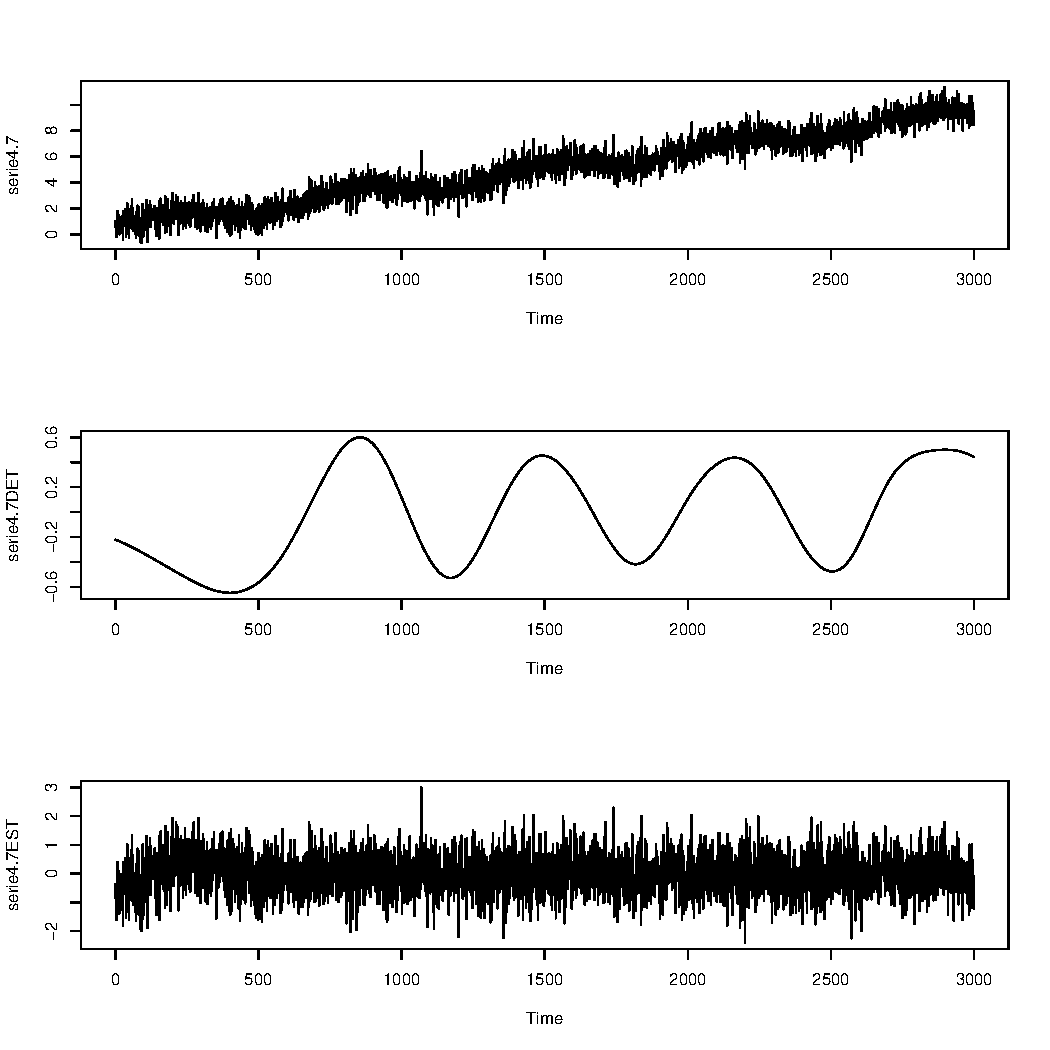
\includegraphics[scale=0.43]{serie4_7.pdf} \quad
  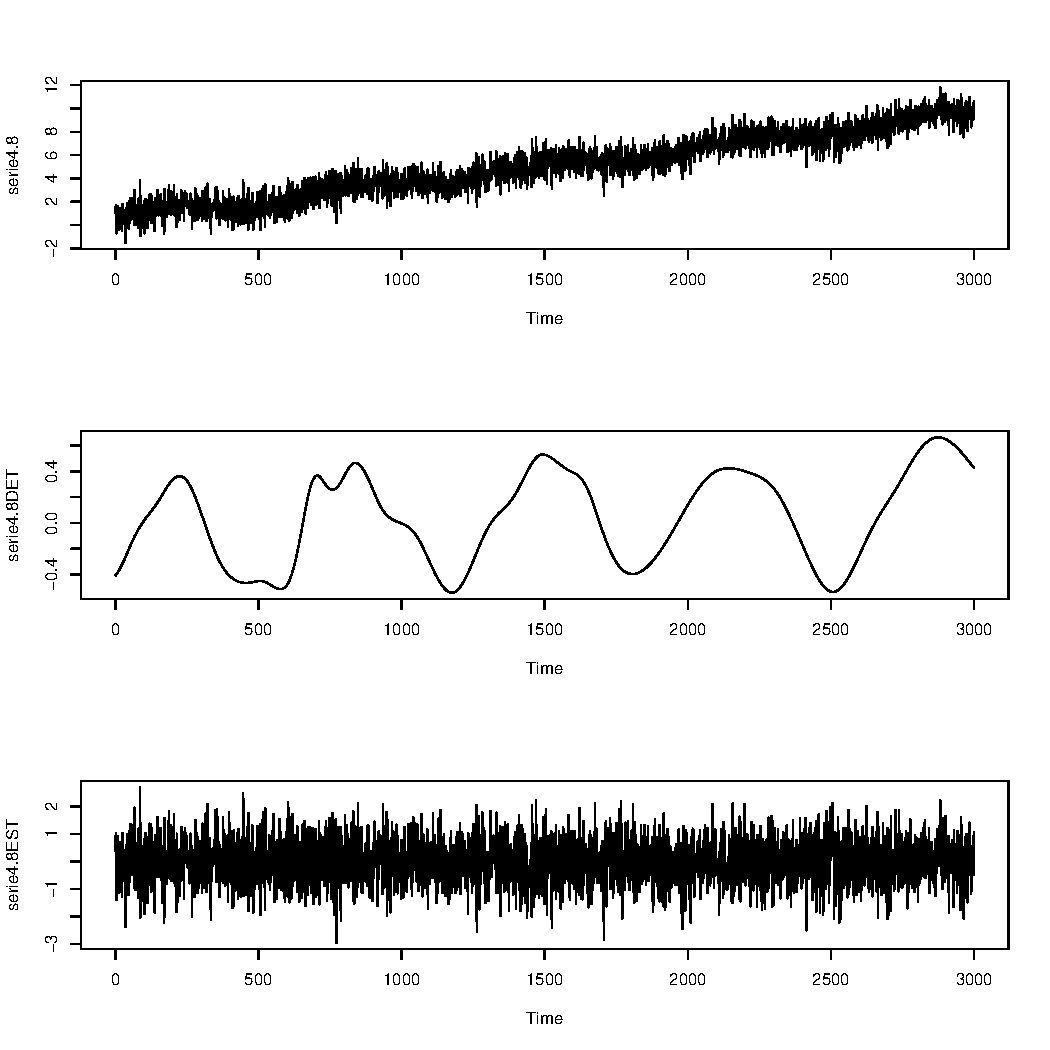
\includegraphics[scale=0.43]{serie4_8.pdf}
  \caption{Série 4.7 e Série 4.8}

\end{center}
\end{figure}

\graphicspath{{imagens/}}
\begin{figure}[H]
\begin{center}
  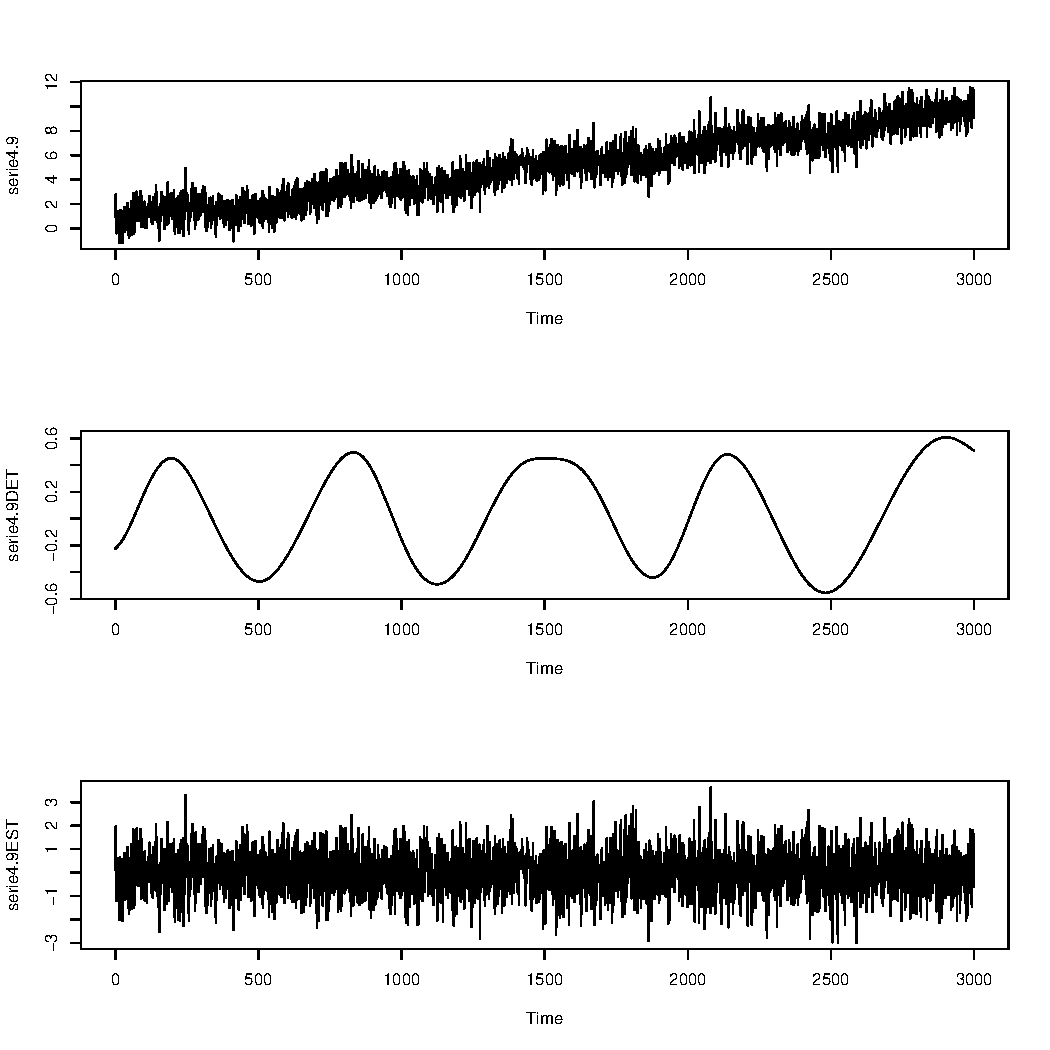
\includegraphics[scale=0.43]{serie4_9.pdf} \quad
  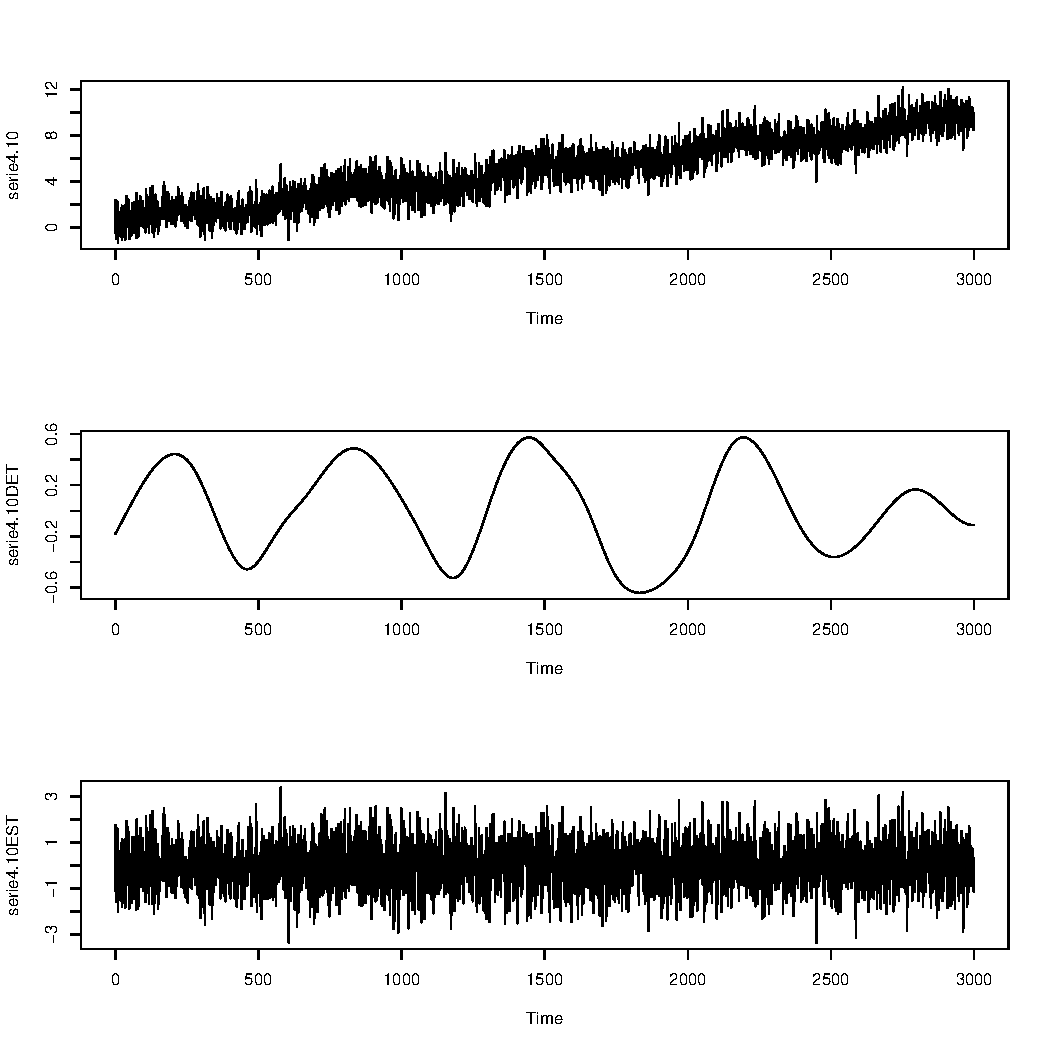
\includegraphics[scale=0.43]{serie4_10.pdf}
  \caption{Série 4.9 e Série 4.10}
\end{center}
\end{figure}
\section{Considerações Finais}
Foram apresentadas as séries temporais utilizadas neste trabalho experimental e suas respactivas decomposições.
% \include{apendice2}
% ...
% \include{apendiceM}

%% Fim do documento
\end{document}
%------------------------------------------------------------------------------------------%
